%%% The main file. It contains definitions of basic parameters and includes all other parts.

%% Settings for single-side (simplex) printing
% Margins: left 40mm, right 25mm, top and bottom 25mm
% (but beware, LaTeX adds 1in implicitly)
\documentclass[12pt,a4paper]{report}
\setlength\textwidth{145mm}
\setlength\textheight{247mm}
\setlength\oddsidemargin{15mm}
\setlength\evensidemargin{15mm}
\setlength\topmargin{0mm}
\setlength\headsep{0mm}
\setlength\headheight{0mm}
% \openright makes the following text appear on a right-hand page
\let\openright=\clearpage

%% Settings for two-sided (duplex) printing
% \documentclass[12pt,a4paper,twoside,openright]{report}
% \setlength\textwidth{145mm}
% \setlength\textheight{247mm}
% \setlength\oddsidemargin{14.2mm}
% \setlength\evensidemargin{0mm}
% \setlength\topmargin{0mm}
% \setlength\headsep{0mm}
% \setlength\headheight{0mm}
% \let\openright=\cleardoublepage

%% Generate PDF/A-2u
\usepackage[a-2u]{pdfx}

%% Character encoding: usually latin2, cp1250 or utf8:
\usepackage[utf8]{inputenc}

%% Prefer Latin Modern fonts
\usepackage{lmodern}

%% Further useful packages (included in most LaTeX distributions)
\usepackage{amsmath}           % extensions for typesetting of math
\usepackage{amsfonts}          % math fonts
\usepackage{amsthm}            % theorems, definitions, etc.
\usepackage{bbding}            % various symbols (squares, asterisks, ...)
\usepackage{bm}                % boldface symbols (\bm)
\usepackage{graphicx}          % embedding of pictures
\usepackage{fancyvrb}          % improved verbatim environment
\usepackage[square]{natbib}    % citation style AUTHOR (YEAR), or AUTHOR [NUMBER]
\usepackage[nottoc]{tocbibind} % makes sure that bibliography and the lists
                               % of figures/tables are included in the table
                               % of contents
\usepackage{dcolumn}           % improved alignment of table columns
\usepackage{booktabs}          % improved horizontal lines in tables
\usepackage{paralist}          % improved enumerate and itemize
\usepackage{xcolor}            % typesetting in color
\usepackage{xurl}
\usepackage{hyperref}
\usepackage{nameref}
\usepackage{macros}
\usepackage{caption}
\usepackage{subcaption}
\usepackage{amsmath}
\usepackage{algorithm}
\usepackage{algpseudocode}
\usepackage{listings}
\usepackage{xcolor}
\usepackage{colortbl}
\usepackage[capitalise]{cleveref}
\usepackage{tikz}
\usepackage{siunitx}
\usetikzlibrary{positioning, graphs, arrows.meta, calc, quotes}
\usepackage[nohyperlinks]{acronym}


\tikzset{process/.style={
    rectangle,
    rounded corners=3mm,
    minimum size=6mm,
    top color=blue!10,
    bottom color=blue!30,
    font=\footnotesize
}}
\tikzset{data/.style={
    rectangle,
    fill=green!20,
    minimum size=6mm,
    align=left,
    font=\footnotesize
}}
\definecolor{darkgreen}{RGB}{0,100,0}


%%% Basic information on the thesis

% Thesis title in English (exactly as in the formal assignment)
\def\ThesisTitle{Evaluating Point Cloud Rendering Approaches for Camera Pose Verification}
\def\NazevPrace{Použití metod zobrazení mračna bodů pro ověření polohy kamery}

% Author of the thesis
\def\ThesisAuthor{Tomáš Kremel}

% Year when the thesis is submitted
\def\YearSubmitted{2024}

% Name of the department or institute, where the work was officially assigned
% (according to the Organizational Structure of MFF UK in English,
% or a full name of a department outside MFF)
\def\Department{Department of Software and Computer Science Education}
\def\Katedra{Katedra softwaru a výuky informatiky}

% Department of Theoretical Computer Science and Mathematical Logic
% Is it a department (katedra), or an institute (ústav)?
\def\DeptType{Department}
\def\TypPracoviste{Katedra}

% Thesis supervisor: name, surname and titles
\def\SupervisorA{doc. Ing. Tomáš Pajdla, Ph.D.}
\def\SupervisorB{Torsten Sattler, Dr. rer. nat.}

% Supervisor's department (again according to Organizational structure of MFF)
\def\SupervisorsDepartment{Department of Algebra}
\def\KatedraVedouciho{Katedra algebry}

% Study programme and specialization
\def\StudyProgramme{Computer Science}
\def\StudyBranch{Artificial Intelligence}

% An optional dedication: you can thank whomever you wish (your supervisor,
% consultant, a person who lent the software, etc.)
\def\Dedication{%
I would like to express my gratitude and appreciation to my supervisors,
for their suggestions, great support, and inexhaustible patience while
I was finding motivation to put this work into reality. I would also like
to thank The Czech Institute of Informatics, Robotics, and Cybernetics
(CIIRC) for providing me with all the
necessary GPU resources required for computations. Lastly, I would like
to recognize my friends Tomáš Souček and Vojtěch Kužel for their consultations.
}

% Abstract (recommended length around 80-200 words; this is not a copy of your thesis assignment!)
\def\Abstract{%
Visual localization is the problem of estimating the 6~degrees of freedom
camera pose from which a query image was taken relative to a known
reference scene representation. It is the key for applications such as
Augmented, Mixed, and Virtual Reality, as well as autonomous robotics
such as drones or self-driving cars.

This thesis focuses on a visual localization pipeline, especially on
its pose verification and reranking step. The pipeline uses 3D point clouds
and 2D-3D correspondences between the query image and 3D scene points for
candidate camera poses estimations. The thesis explores point cloud
rendering approaches as they are utilized in the pipeline and the
verification step---the render of the discretized scene from a given
candidate position is compared to the actual query image to asses if the
given couple depicts the same place.

One of the main challenges of such rendering is occlusion handling. Due
to the sparsity of points employed for otherwise continuous real world
representation, information about what lies in the front and what is
hidden can be easily lost when projected to the 2D image. Rendering
approaches explored in this thesis focus on the challenge directly or
as a component of a novel view synthesis DNN-based renderer.
Rendering influence on localization performance is investigated.
}

% 3 to 5 keywords (recommended), each enclosed in curly braces
\def\Keywords{%
{point clouds,} {rendering,} {neural rendering,} {localization}
}

\def\Abstrakt{%
Vizuální lokalizace je problém odhadování parametrů šesti stupňů volnosti
pozice kamery, z~níž byla pořízena dotazovaná fotografie, přičemž pozice
je vztažena ke známé reprezentaci referenčního prostředí. Řešení tohoto
problému je klíčové v~aplikacích jako jsou rozšířená, smíšená a~virtuální
realita, stejně tak v~oblasti autonomní robotiky zahrnující drony
a~samořiditelné automobily.

Tato práce se soustředí na vizuální lokalizačního algoritmus, zejména na
jeho verifikační a~přeřazovací krok. Tento algoritmus interně využívá
tří dimenzionální mračna bodů a~hledání korespondencí mezi těmito body
a~dotazovanou fotografií pro nalezení odhadů kandidátních pozic kamery.
Práce zkoumá přístupy k~renderování mračen bodů a jejich využití v~rámci
algoritmu a jeho verifikačního kroku~-- render diskretizovaného prostředí
z~konkrétní kandidátní pozice se v něm porovnává s~danou dotazovanou fotografií
za účelem určení toho, zda oba pohledy zobrazují to samé místo.

Jedna z~hlavních výzev renderingu diskretizovaného prostředí jsou okluze.
Kvůli řídkosti bodů využitých jako reprezentace jinak spojitého reálného
světa může být informace o~tom co leží v~popředí a co v~pozadí lehce
ztracena při promítnutí bodů na dvou dimenzionální obraz. Přístupy
k~renderování zkoumané v~této práci se soustředí na renderování bodů přímo
nebo jako komponentu rendereru \uv{nových pohledů} využívající hlubokých
neuronových sítí. Je zde prověřen vliv těchto renderovacích přístupů na
přesnost lokalizace.
}

\def\KlicovaSlova{%
{mračna bodů,} {rendering,} {neurální rendering,} {lokalizace}
}

%% The hyperref package for clickable links in PDF and also for storing
%% metadata to PDF (including the table of contents).
%% Most settings are pre-set by the pdfx package.
\hypersetup{unicode}
\hypersetup{breaklinks=true}

% Definitions of macros (see description inside)
% %%% This file contains definitions of various useful macros and environments %%%
%%% Please add more macros here instead of cluttering other files with them. %%%

%%% Minor tweaks of style

% These macros employ a little dirty trick to convince LaTeX to typeset
% chapter headings sanely, without lots of empty space above them.
% Feel free to ignore.

\ProvidesPackage{macros}[2022/01/10 v1.0 Thesis macros]

\makeatletter
\def\@makechapterhead#1{
  {\parindent \z@ \raggedright \normalfont
   \Huge\bfseries \thechapter. #1
   \par\nobreak
   \vskip 20\p@
}}
\def\@makeschapterhead#1{
  {\parindent \z@ \raggedright \normalfont
   \Huge\bfseries #1
   \par\nobreak
   \vskip 20\p@
}}
\makeatother

% This macro defines a chapter, which is not numbered, but is included
% in the table of contents.
\def\chapwithtoc#1{
\chapter*{#1}
\addcontentsline{toc}{chapter}{#1}
}

% Draw black "slugs" whenever a line overflows, so that we can spot it easily.
\overfullrule=1mm

%%% Macros for definitions, theorems, claims, examples, ... (requires amsthm package)

\theoremstyle{plain}
\newtheorem{thm}{Theorem}
\newtheorem{lemma}[thm]{Lemma}
\newtheorem{claim}[thm]{Claim}

\theoremstyle{plain}
\newtheorem{defn}{Definition}

\theoremstyle{remark}
\newtheorem*{cor}{Corollary}
\newtheorem*{rem}{Remark}
\newtheorem*{example}{Example}

%%% An environment for proofs

\newenvironment{myproof}{
  \par\medskip\noindent
  \textit{Proof}.
}{
\newline
\rightline{$\qedsymbol$}
}

%%% An environment for typesetting of program code and input/output
%%% of programs. (Requires the fancyvrb package -- fancy verbatim.)

\DefineVerbatimEnvironment{code}{Verbatim}{fontsize=\small, frame=single}

%%% The field of all real and natural numbers
\newcommand{\R}{\mathbb{R}}
\newcommand{\N}{\mathbb{N}}

\newcommand{\CC}{C\nolinebreak\hspace{-.05em}\raisebox{.4ex}{\tiny\bf +}\nolinebreak\hspace{-.10em}\raisebox{.4ex}{\tiny\bf +}}

%%% Useful operators for statistics and probability
\DeclareMathOperator{\pr}{\textsf{P}}
\DeclareMathOperator{\E}{\textsf{E}\,}
\DeclareMathOperator{\var}{\textrm{var}}
\DeclareMathOperator{\sd}{\textrm{sd}}

%%% Transposition of a vector/matrix
\newcommand{\T}[1]{#1^\top}

%%% Various math goodies
\newcommand{\goto}{\rightarrow}
\newcommand{\gotop}{\stackrel{P}{\longrightarrow}}
\newcommand{\maon}[1]{o(n^{#1})}
\newcommand{\abs}[1]{\left|{#1}\right|}
\newcommand{\dint}{\int_0^\tau\!\!\int_0^\tau}
\newcommand{\isqr}[1]{\frac{1}{\sqrt{#1}}}
\newcommand*{\fullref}[1]{\hyperref[{#1}]{\cref*{#1}: \nameref*{#1}}}

%%% Various table goodies
\newcommand{\pulrad}[1]{\raisebox{1.5ex}[0pt]{#1}}
\newcommand{\mc}[1]{\multicolumn{1}{c}{#1}}

%%% Other macros
\renewcommand{\labelitemi}{\footnotesize{\textbullet}}
\newcommand{\uv}[1]{``#1''}
\newcommand{\footnotei}[2]{%
\setbox0\hbox{#1}%
\copy0%
\hspace{-\wd0}%
\footnote{#2}%
}

\newcommand{\gear}[6]{%
  (0:#2)
  \foreach \i [evaluate=\i as \n using {\i-1)*360/#1}] in {1,...,#1}{%
    arc (\n:\n+#4:#2) {[rounded corners=1.5pt] -- (\n+#4+#5:#3)
    arc (\n+#4+#5:\n+360/#1-#5:#3)} --  (\n+360/#1:#2)
  }%
  (0,0) circle[radius=#6]
}

\makeatletter
\newcommand{\gettikzxy}[3]{%
  \tikz@scan@one@point\pgfutil@firstofone#1\relax
  \edef#2{\the\pgf@x}%
  \edef#3{\the\pgf@y}%
}
\makeatother


% Title page and various mandatory informational pages
\begin{document}
%%% Title page of the thesis and other mandatory pages

%%% Title page of the thesis

\pagestyle{empty}
\hypersetup{pageanchor=false}
\begin{center}

\centerline{\mbox{\includegraphics[width=166mm]{../graphics/logo-en.pdf}}}

\vspace{-8mm}
\vfill

{\bf\Large MASTER THESIS}

\vfill

{\LARGE\ThesisAuthor}

\vspace{15mm}

{\LARGE\bfseries\ThesisTitle}

\vfill

\Department

\vfill

{
\centerline{\vbox{\halign{\hbox to 0.45\hsize{\hfil #}&\hskip 0.5em\parbox[t]{0.45\hsize}{\raggedright #}\cr
Supervisor of the master thesis:&\Supervisor \cr
\noalign{\vspace{2mm}}
Study programme:&\StudyProgramme \cr
\noalign{\vspace{2mm}}
Study branch:&\StudyBranch \cr
}}}}

\vfill

% Zde doplňte rok
Prague \YearSubmitted

\end{center}

\newpage

%%% Here should be a bound sheet included -- a signed copy of the "master
%%% thesis assignment". This assignment is NOT a part of the electronic
%%% version of the thesis. DO NOT SCAN.

%%% A page with a solemn declaration to the master thesis

\openright
\hypersetup{pageanchor=true}
\pagestyle{plain}
\pagenumbering{roman}
\vglue 0pt plus 1fill

\noindent
I declare that I carried out this master thesis independently, and only with the cited
sources, literature and other professional sources. It has not been used to obtain another
or the same degree.

\medskip\noindent
I understand that my work relates to the rights and obligations under the Act No.~121/2000 Sb.,
the Copyright Act, as amended, in particular the fact that the Charles
University has the right to conclude a license agreement on the use of this
work as a school work pursuant to Section 60 subsection 1 of the Copyright~Act.

\vspace{10mm}

\hbox{\hbox to 0.5\hsize{%
In \hbox to 6em{\dotfill} date \hbox to 6em{\dotfill}
\hss}\hbox to 0.5\hsize{\dotfill\quad}}
\smallskip
\hbox{\hbox to 0.5\hsize{}\hbox to 0.5\hsize{\hfil Author's signature\hfil}}

\vspace{20mm}
\newpage

%%% Dedication

\openright

\noindent
\Dedication

\newpage

%%% Mandatory information page of the thesis

\openright

\vbox to 0.5\vsize{
\setlength\parindent{0mm}
\setlength\parskip{5mm}

Title:
\ThesisTitle

Author:
\ThesisAuthor

\DeptType:
\Department

Supervisor:
\Supervisor, \SupervisorsDepartment

Abstract:
\Abstract

Keywords:
\Keywords

\vss}

\newpage

\openright
\pagestyle{plain}
\pagenumbering{arabic}
\setcounter{page}{1}


%%% A page with automatically generated table of contents of the master thesis

\tableofcontents

%% Each chapter is kept in a separate file
\chapter*{Introduction}
\addcontentsline{toc}{chapter}{Introduction}


\chapter{Visual Localization} \label{chap:visual_loc}

As stated in~\nameref{intro}, visual localization is the task of finding
the position of a camera that took a query photo relative to a reference scene
representation, and it is one of the fundamental problems in computer vision.

Compared to network-based localization methods, such as GNSS, visual localization,
even though being able to work in network-denied environments, comes with its own
set of problems that any successful method must consider. For both outdoor and
indoor localization, to which the field is typically separated due to different
localization complexity, illumination changes throughout the day and artificial lighting
influence present in the environment's representation data pose one class of such problems.
Further, it must cope with transient dynamic objects that can be present in both query
and database data, possibly occluding important feature-rich areas but having nothing
to do with the long-term visual appearance of the given location. Outdoors, seasonal and
weather-caused changes must be handled as well. For indoors, more problems stem from
textureless areas such as walls, ceilings, and floors; from repetition and symmetry
on both the global level with corridors, for example, and the local level, such as door handles.
Also, compared to outside, with typically longer distances between objects, inside small change
of viewing position leads to a vastly different view.

In this chapter, we present previous work on the matter and describe the InLoc method
explored in the thesis, explaining why this very method is chosen.

\section{Related work}

There are three main method categories for visual localization, as of \citet{torsten2018},
\citet{torsten2019}, \citet{torsten2021}, \citet{naverlabs}: methods based on structure,
image retrieval, and pose regression.

\subsubsection*{Structure-based methods}

Structure-based methods are the traditional way of estimating poses where a 3D model (the \emph{structure}) is
pre-created in order to later find 2D-3D correspondences.

% used https://arxiv.org/pdf/2007.13867.pdf
The 3D model is typically created by
Structure-from-Motion~\citep{SfM, schoenberger2016mvs}, by computing local sparse features (keypoints with descriptors,
\citet{LoweLocalization} used SIFT~\citep{SIFT} descriptor, \citet{PreSIFT} was pre-SIFT, using image rectification)
per database image with known focal length, match them against each other across images, and triangulate resulting 3D points
from these matches. Since the model already contains pre-computed features, matching against
a query image's features can then be performed. Since the 2D-3D matches are determined, the camera pose
is computed using the perspective-n-point (PNP) solver~\citep{PnP}. Because of the possible presence of outlier matches,
a RANSAC loop~\citep{RANSAC} is utilized to increase robustness. Other examples of this approach are~\citet{2D3D, 2D3D_2}.

With the growing size of a 3D point cloud, the runtime gets prolonged. To mitigate matching speed deterioration,
these methods also get paired with image retrieval, described next, to find the most
relevant images from the SFM model. Examples of these methods
are~\citet{InLoc, InLocRevisited, MegLoc}.

\subsubsection*{Image retrieval-based methods}

Image retrieval can be used to speed up the structure-based method family and make mapping
and localization more robust. That is because the restriction of matching to the parts of the scene visible in the given query photo
helps to avoid global ambiguities in the scene, e.g., caused by similar structures found in unrelated parts
of a scene~\citep{InLocRevisited}. It can also be used on its own for a closely related task to visual
localization called place recognition, which strives to find the approximate location of a query photo within a database
of geo-tagged images. Unlike visual localization, place recognition
does not need an explicit model representation, so no depth values nor point clouds are necessary for these
methods to work. Because of less input information, the location obtained by the retrieval and interpolating of several geo-tags
or camera poses is, in general, less accurate~\citep{InterpolationRetrieval, RegressionPose}.

In both cases, the goal is to gather a set of images that are the most similar according to a selected
criterion---here, a retrieved image is considered relevant if it sees the same scene---followed by an
optional re-ranking step. Historically, image retrieval methods have used variants of Bag of Visual Words~\citep{BoVW}
and Vector of Locally Aggregated Descriptors (VLAD)~\citep{VLAD},
newer approaches utilize features extracted by a Deep Neural Network (DNN) as such features encode high-level semantics
better than sparse features such as SIFT~\citep{RetrievalEE, DNNRegression, hausler2021patchnetvlad}.

\subsubsection*{Pose regression-based methods}

This category of methods uses a DNN for regressing the query pose end-to-end from an RGB image
directly to a 6~DoF pose. Based on the assumption that features obtained by a Neural Network (NN) trained for a general vision task
also include some helpful information for pose estimation, transfer learning is leveraged for the pose regression.

% https://arxiv.org/pdf/2207.05530.pdf
PoseNet~\citep{PoseNet} is an example of such an approach using an image classification CNN architecture, like
VGGNet or ResNet, with fully connected layers to regress the pose at the end of the architecture. Regression-based
methods are generally less accurate than structure-based localization (for PoseNet, by order of magnitude).
However, their advantage lies in short, constant inference time and smaller memory and computation power requirements
using just a single forward pass, even without requiring the camera intrinsics parameters, which may be
inaccurate and unavailable~\citep{RegressionAutoEnc}. The accuracy problem is inherent here, as end-to-end
learning imposes a tight coupling with the database coordinates. Thus, such a network can be seen as a compressed
version of the database itself, which limits the generalization power of the network~\citep{naverlabs}. As the approach is still
interesting for other use cases, many improvements were presented, such as~\citet{DNNRegression, Maps, VLocNet}
and~\citet{VLocNetpp}.


\section{InLoc}\label{sec:inloc}
This visual localization method, so-called \emph{Indoor Visual Localization with Dense Matching
and View Synthesis}, falls amid two-staged structure-based approaches combined with image retrieval. The first stage finds
correspondences between a query image features and model of a scene, and the second estimates the camera pose.
The method's input is a database of RGBD
images with known focal lengths (from EXIF data, for instance), and the method internally uses a point cloud 3D scene
representation. The method focuses on indoor localization and addresses several
issues presented in~\nameref{intro}. Visual representation of the method with a short summary can be seen in~\cref{fig:inloc_intro}.

\begin{figure}
    \centering
    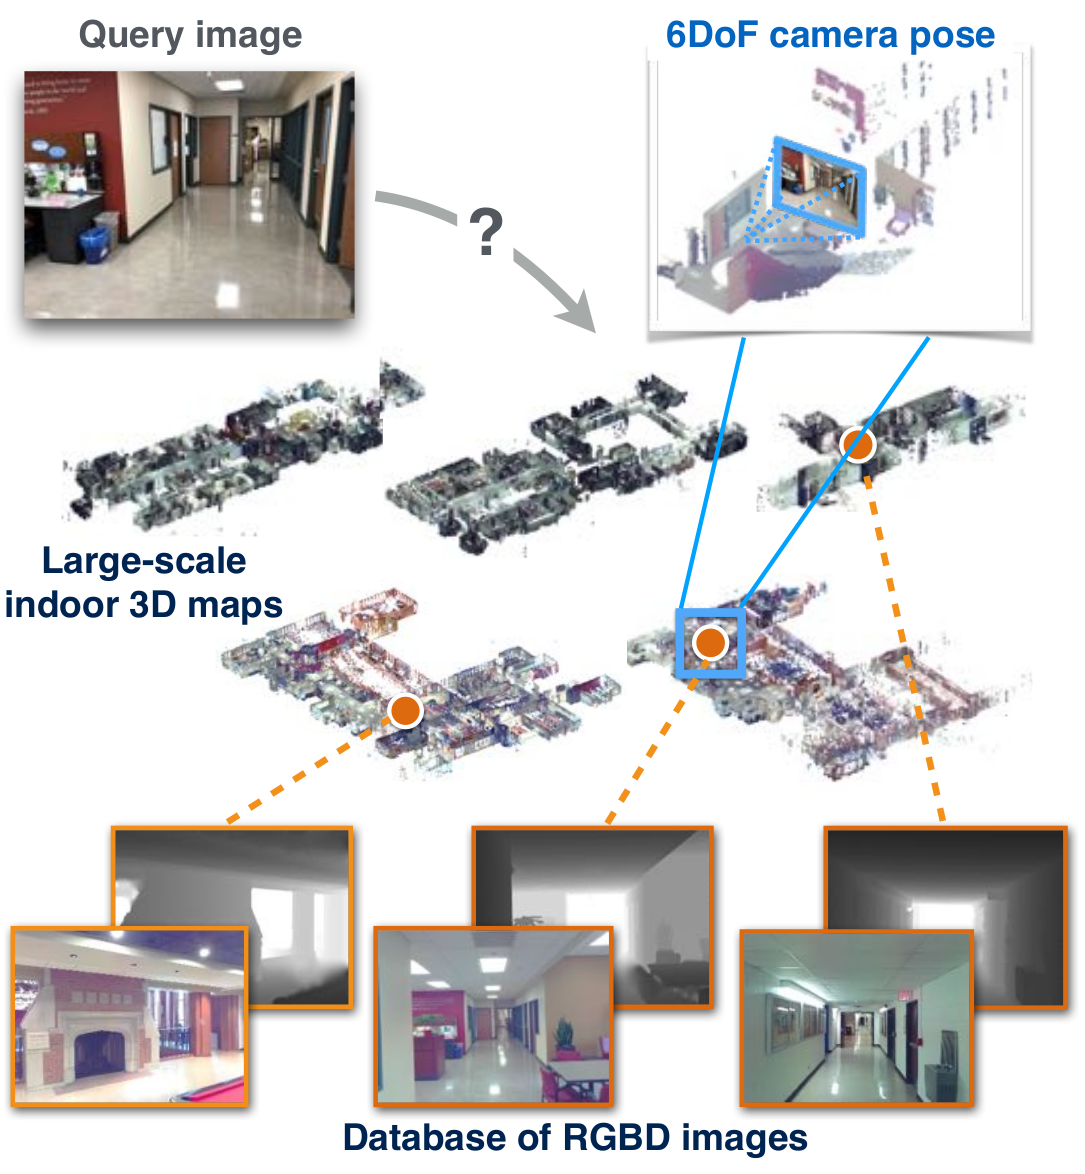
\includegraphics[width=.5\textwidth]{../graphics/inloc.png}
    \caption[InLoc explained]{Given a database of geometrically-registered RGBD images, InLoc predicts
    the 6~DoF camera pose of a query RGB image by retrieving candidate images, estimating candidate camera poses, and selecting
    the best matching camera pose. Image taken from~\citet{InLoc}.}\label{fig:inloc_intro}
\end{figure}

All of illumination changes~(1), textureless areas~(3) leading to lack of sparse local features, such as SIFT~\citep{SIFT},
repetitive elements in indoor settings~(4) leading to similar repetitive features being produced, and even viewpoint changes~(5)
are overcome by utilizing multi-scale dense CNN features computed densely on a regular grid by NetVLAD~\citep{NetVLAD}.
These features are used for database image retrieval, as $N=100$ best matching images are chosen based on sorted
normalized L2 distances of the extracted database feature vectors and the query feature vector.

In the next stage, candidate images are re-ranked by another feature matching in the geometric verification process and
pose estimation. Firstly, features are extracted by VGG~\citep{VGG16} model on conv5 and subsequently on conv3 layer
restricted by previously found matches are used for finding geometrically consistent sets of correspondences with
RANSAC~\citep{RANSAC}. Based on the number of RANSAC inliers, top $M = 10$ candidate database images are kept.
It is to be noted that these features are obtained with no additional computation burden as VGG is used internally
by NetVLAD. As database images used as input to the method are RGBD and hence they have associated 3D points, the
query camera pose is then estimated by finding pixel-to-pixel correspondences between the query and the top
$M$~database images followed by P3P-LO-RANSAC~\citep{P3PLORANSAC}.

To further cope with self-similarity found in indoor locations, counting the number of inliers
as positive evidence to decide whether two views are taken from an exact location is not the
only decisive criterion. Negative evidence is also used in the form of the portion of the view
rendered from the candidate query pose that does not match the query photo. Authors of the paper
refer to this as \emph{explicit pose estimate verification based on view synthesis}. Verification
is done pixel-wise to obtain consistent and inconsistent pixels between the render and the query photo.
To keep invariance to illumination changes and small misalignments, pixel comparison operates with RootSIFT
local patch descriptors~\citep{RootSIFT}. The final image-render similarity is the median of descriptor distance
across the entire image while ignoring areas with missing 3D structure resulting in background-filled regions in renders.

This thesis further examines the view synthesis part of the verification process as it changes the rendered source imputed
to the RootSIFT descriptor computation process. In further chapters, three rendering
techniques alternative to the baseline \verb|GL_POINTS| rendering approach are described in detail.

The decision to use the InLoc method in the thesis was driven by the fact that it is the first method of its kind,
state-of-the-art of its time that puts basis or plays a role of a baseline for
other subsequent state-of-the-art methods~\citep{PoseCorrection}. Further, its source codes are public\footnotei{,}{\url{http://www.ok.sc.e.titech.ac.jp/INLOC}} whereas a subsequent paper~\citep{InLocRevisited}
presenting some improvements does not provide source codes.

\chapter{Point Cloud Rendering} \label{chap:pcd_rendering}

As stated in~\citet{PointRendering}, using point primitives for rendering has been driven
by two main reasons. Over the years,
there was a dramatic increase in the polygonal complexity of models being rendered, leading to
the overhead of managing and processing extensive mesh connectivity information.
Further, modern 3D scanners (LiDAR, stereo camera setup) or photogrammetry methods (SfM) produce
both geometry and appearance of complex, real-world objects in the form of a point cloud. Points in a point cloud
play the role of (discrete) building blocks for 3D scenes, similar to how pixels are the digital ones for images.

Points are the simplest graphic primitive, generalizing pixels towards irregular samples of
geometry and appearance. They differ from triangles typically used in computer graphics
by carrying all attributes needed for processing and rendering with themselves the same way
as pixels do. That results in transformation of rendering pipeline, the terms vertex and fragment coincide in
one entity. Even though the presence of just one such entity may lead to simpler graphical pipelines,
it is not without issues~\citep{ComputeShaderRendering}.

1) Straightforward points projection leaves empty spaces in the image that need to be filled
for close-up views as it may lead to problems with occlusions and visibility or depth perception---with
less dense sampling, a render can end up with just many points scattered across
the background with no notion of what is closer and farther. Thus, point clouds typically
require a denser sampling compared to triangle meshes. 2) Points do not possess any topology or
connectivity information. This fact is an advantage and disadvantage at the same time, compared to
meshed that contain this type of information, but only as a result of 3D reconstruction
algorithms with point clouds being an input that typically still require some prior assumptions on topology
and sampling. It is, for instance, possible to stream and render point clouds progressively, and
change of topology (e.g., by filtering) is more straightforward than for meshes where one needs to recompute
connectivity information~\citep{PointRendering}. On the other hand, effective point processing typically needs
elaborate data structures, including KD-trees~\citep{KDTree} or spatial hashing~\citep{SpatialHashing}.

Over the years, many approaches have been devised for processing point primitives and tackling the
issues presented in the preceding paragraphs. In the thesis, we take advantage of having point clouds-based
datasets. We found out that for large indoor areas, it may be tricky to come up with sufficiently good
mesh that can be further used for the localization verification step rendering, as it can be seen
in~\cref{fig:mesh_artwin_render}. Proceeding with point cloud-based rendering techniques,
we work with three of them together with the mentioned baseline \verb|GL_POINTS| approach;
see their descriptions in the following sections.

\begin{figure}
    \centering
    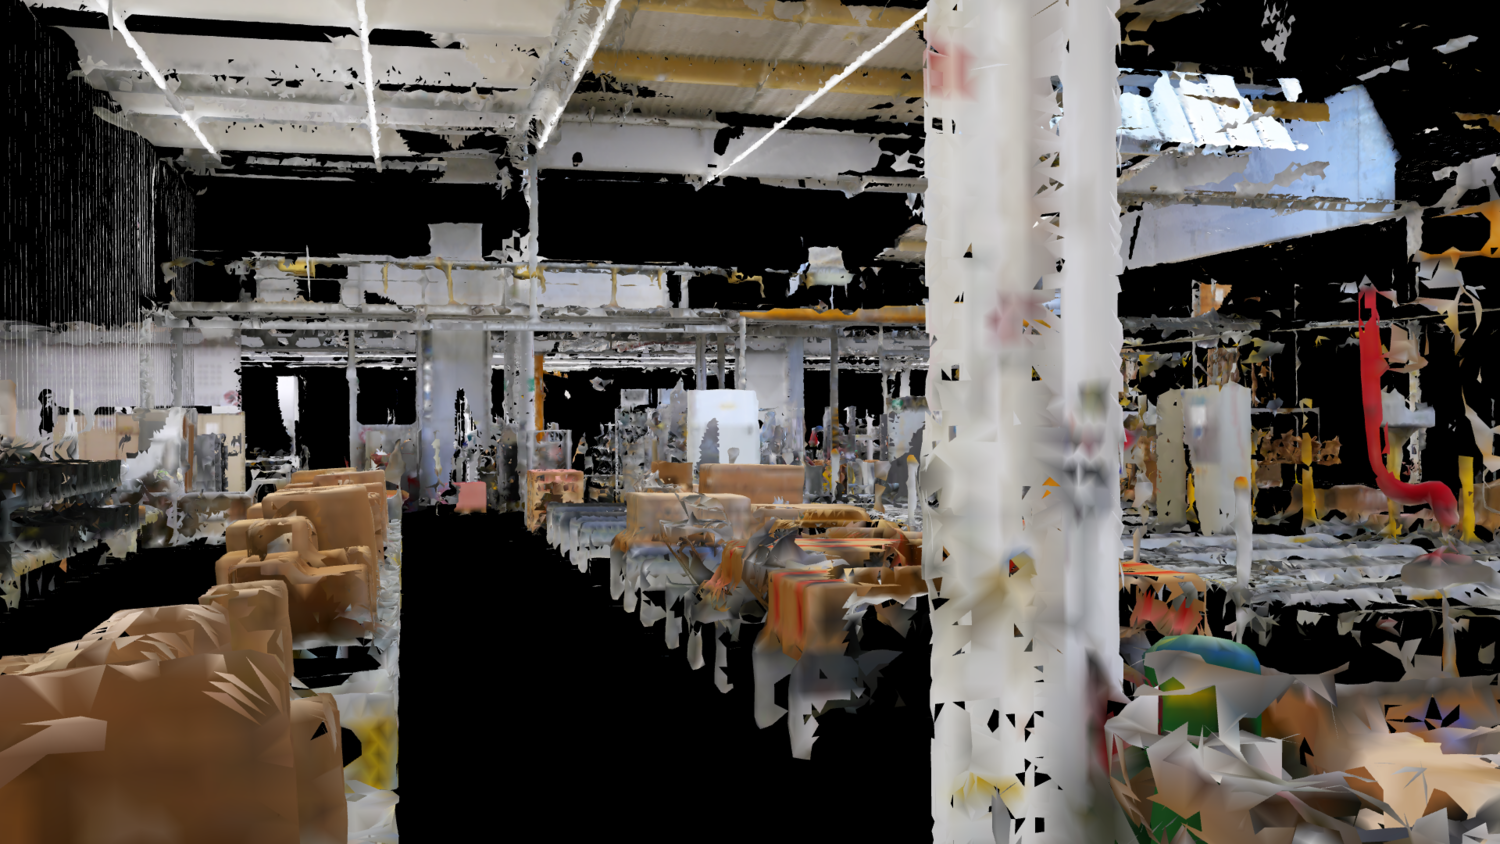
\includegraphics[width=.9\textwidth]{../graphics/0217_mesh_artwin_render.png}
    \caption[ARTwin mesh rendered view]{A render of one of the meshes created from the raw datasets' point cloud, camera pose is the same
    as for~\cref{fig:pyrender_artwin_render}. The mesh was created
    semi-manually, meaning that boxes, for instance, were meshed separately and then placed at the right
    place of the resulting mesh. We can see some disadvantages of using meshes in complex environments.
    Despite long processing time and laborious manual work, the result is not compelling compared to renders
    using point primitives.}\label{fig:mesh_artwin_render}
\end{figure}

\section{Related Work}

\citet{SOTARendering} defined \emph{rendering} as transforming a scene definition, including some of the cameras,
lights, surface geometry, and material, into a simulated camera image. The process can be organized in two
ways~\citep{marschner2021fundamentals}. \emph{Object-order} rendering considers each object; for such,
all the pixels it influences are found and updated. In \emph{image-order} rendering, the loop
goes the other way round, each pixel is considered, and for such, all the objects that influence it are found, and
the pixel value is computed. From these two approaches, image-order rendering is simpler to implement and more capable in the
effects that can be incorporated and usually (though not always) takes more execution time compared to the second approach.
Object-order rendering is also known as \emph{rasterization}, whereas under
\emph{image-order} rendering, there are more possible approaches, such as ray-casting and ray-tracing.\\

Rasterization is typically hardware-accelerated because it has good memory coherence~\citep{SOTARendering}, which is also
one of the reasons for one of the previous claims about execution speed comparison. (Though modern GPU cards already have
hardware support for ray-tracing as well\footnotei{.}{\url{https://developer.nvidia.com/rtx/ray-tracing}}) The rasterization,
as a representative of the object-order methods, requires an explicit scene representation, such as mesh or point cloud, whereas the other
methods work with both implicit and explicit representations.\\

Ray-casting and ray-tracing are, in some sense, orthogonal methods within image-order realm; see~\cref{fig:casting_tracing}.
Ray-casting computes a ray (coming from the camera center
through a specific pixel of the screen) intersections with the representation of the scene to project the scene onto the screen.
In ray-tracing, the primary ray is considered to be coming from the scene, through the screen to the camera center, conveying
color information gathered from all physics-based interactions of light with objects in the scene. Reflections and refractions
are simulated by recursively casting new rays from the intersections with the geometry~\citep{Whitted1979AnII}. The advantage
of this rendering process is the realism of the simulation of real-world optical effects.
While rasterization and ray-casting are a simple, one-way
processes, ray-tracing is an inherently recursive problem. Hence it is a more complex task.

\begin{figure}
    \centering
    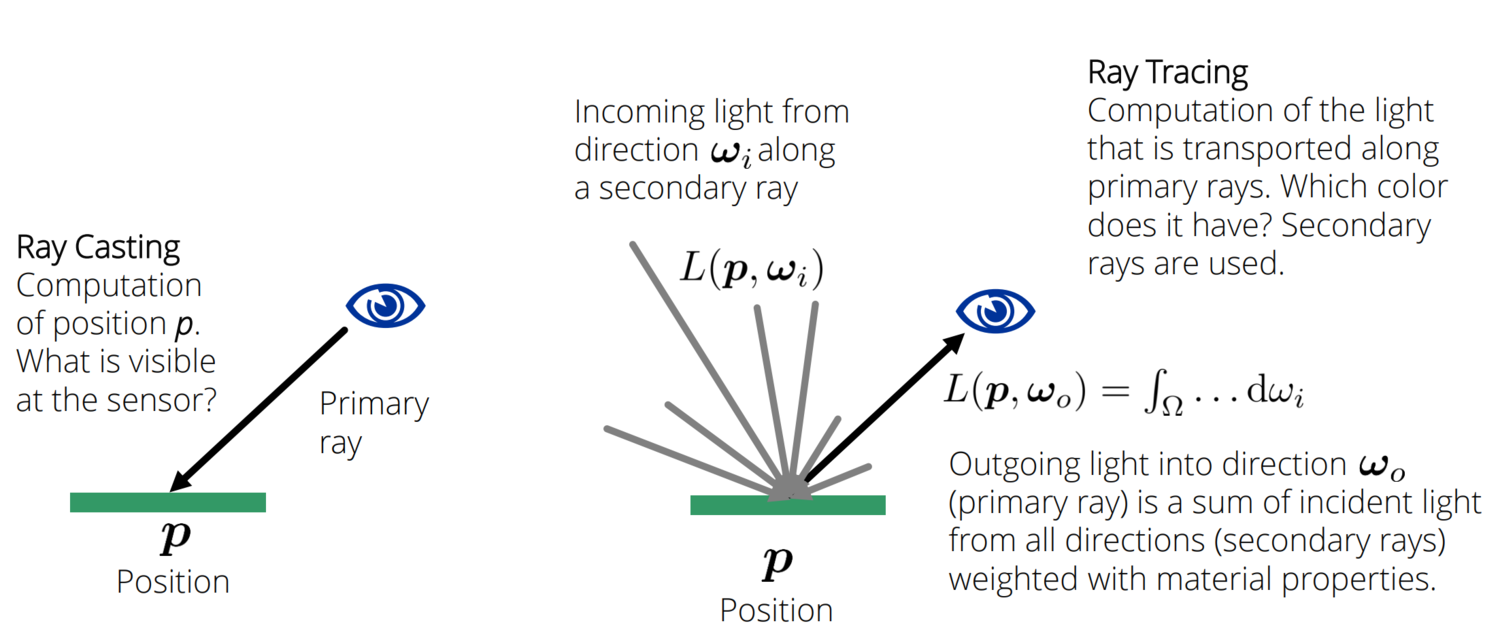
\includegraphics[width=.9\textwidth]{../graphics/casting-tracing.png}
    \caption[Ray-casting vs. ray-tracing]{A demonstration of the difference between
    ray-casting and ray-tracing, together with an illustration of the recursive nature
    of the ray-casting algorithm. Taken from~\url{https://cg.informatik.uni-freiburg.de/course_notes/graphics_01_raycasting.pdf}.}\label{fig:casting_tracing}
\end{figure}

For rendering points with the classical approaches, surface splatting was proposed as a forward-projection approach that uses a z-buffer
algorithm for visibility resolution of points that are exchanged for oriented ellipses. Splatting can process point clouds
without additional acceleration data structures such as spatial hierarchies, which are
often required in ray-tracing approaches~\citep{PointRendering}. The initial article is mainly
a mathematical model and a CPU demonstrator that was later revisited by several papers that enhanced some of its
features and ported it to GPUs~\citep{Splatting2, Splatting3, Splatting4, Splatting5, Splatting6}.
Splatting can also be enriched with ray-tracing again to simulate more complex visual effects~\citep{SplattingTracing}.
Also, further GPU-related enhancements were proposed with better data structures suited for the usage~\citep{SequentialTrees}.\\

Another family of methods takes a vastly different approach than the classical rendering described
above---while traditional computer graphics
methods focus on modeling scenes from a physics perspective, simulating light transport and other effects,
machine learning can be used for modeling the distribution of real-world imagery. The models utilized for this task
are called generative models, successors of the work on \emph{Generative Adversarial Neural Networks}
(GANs)~\citep{GAN}, and can generate high-resolution images~\citep{ICLR, ICLR2} or videos~\citep{VPT, CDS}.
More specifically, the field of so-called neural rendering
combines generative machine learning techniques with knowledge from classical computer
graphics. It is defined as \uv{deep image or video generation approaches that enable
explicit or implicit control of scene properties such as illumination, camera parameters, pose, geometry, appearance,
and semantic structure}~\citep{SOTARendering}. GANs produce \emph{random}, realistically-looking images that resemble
the training set~\citep{DGM} statistically. As the definition of neural rendering states, user controllability
is important---if used by an artist, outputs reflecting design ideas are preferred over some random imagery.
For applications in the neural rendering field, GANs thus needed to be extended by the conditioning of output
to enable guidance of the rendering process.

Further citing~\citet{SOTARendering}, neural rendering techniques can be classified along different axes:
\begin{itemize}
    \item \textbf{Control}. This axis distinguishes neural rendering approaches based on
    what properties from the definition are controllable and how they condition
    the network's output. A general solution enabling to control everything is an open
    research problem. Typically only a subset of controllable properties is approached
    in subproblems like novel view synthesis, relighting, or face and bodies animation.
    The conditioning can be performed by passing the scene parameters as input to some network
    layer or concatenating them to activations of an inner one, by tiling scene parameters over
    all pixels of an input image resulting in packed input volume, it can also employ
    an image-to-image transformation DNN that fuses \uv{guide image} into to the output one.
    Also, a more traditional approach uses scene parameters as an input to a graphical layer.
    \item \textbf{Computer Graphics Modules}. The separation along this axis is based on how much
    of the classical rendering pipeline is integrated into the specific method. The simplest way
    to achieve that is to use a non-differentiable computer graphics (CG) component in the network
    architecture, which would present the render as an input to subsequent differentiable layers of a given architecture.
    When the module is at the beginning of the architecture, the task transforms into
    well-researched image-to-image translation. Fully differentiable CG modules also exist.
    \item \textbf{Explicit vs. Implicit Control}. Here, the criterion is based on a type of
    control signal. Explicit control from a user perspective means manual editing capability
    of scene parameters in a semantically meaningful manner. By implicit control, a representative
    sample as input is meant. The difference also translates to training data as explicit control
    needs richer annotations, whereas implicit one performs well with less supervision.
    \item \textbf{Multi-modal Synthesis}. Not only from an art perspective, often it is beneficial to have
    multiple outputs from which a user can choose. Especially when only a subset of scene properties is
    controllable, within the rest, there lies an output space of possible results from which a given model
    can sample. This sampling capability adds complexity to the architecture, requiring some
    stochasticity or structured variance built-in, leading to GAN or variational auto-encoders (VAEs) variants.  % TODO clanek
    \item \textbf{Generality}. Does the rendering approach perform well over multiple
    scenes or objects without retraining the underlying model? Object-specific approaches
    still produce higher quality outputs at the cost of lengthy per-instance retraining. General models
    are still an open research area.
\end{itemize}

Methods spread across this classification landscape solve various subtasks of the neural rendering field.
Given the model this thesis utilizes, the novel view synthesis task is described next.\\

\emph{Novel view synthesis} generates a view of a
scene, represented by a fixed set of input images, from previously unexplored camera poses. Challenges tied to this task are inferring the scene's 3D
representation, given sparse observations in the form of images and deducing of occluded
or unseen areas of the scene. For the scene reconstruction, the aforementioned SfM is being utilized, followed by
MultiView Stereo (MVS)~\cite{MVS1, MVS2} or variational optimization~\cite{VarOpt}.

The classical computer vision approach towards novel view synthesis utilizes so-called image-based rendering (IBR)
methods~\citep{IBR1, IBR2, IBR3, IBR4} where views from new viewports are generated by warping input pixels into the
outputs using proxy geometry. These methods are sensitive to the scene database size as IBR may fail with insufficient number of source photos, resulting in ghosting-like artifacts and holes~\citep{SOTARendering}. These approaches
also do not handle multiple appearances well~\citep{NRIW}. Neural networks and
rendering alternative approaches have been proposed to mitigate these issues, such as~\citet{NR1, NR2, NRIW, InvSfM, FVS, SVS}.
These methods build on IBR and image-to-image translation using explicit scene models. Learned implicit
scene representation can be leveraged as well, see the Neural Radiance Fields~\citet{NERF, NERF2}
and~\citet{SceneRepr}.

The Neural Radiance Fields, together with the Gaussian Splatting neural model~\citep{kerbl3Dgaussians}
combining the neural field with the splatting idea explored in the thesis represent the recent progress
in the field nicely, alleviating some of the issues of the previous models. However, they were not yet
available when the work on the thesis was started, they are not considered.


\section{Neural Rerendering In the Wild}

According to the neural rendering techniques classification, the \emph{Neural Rerendering In the Wild} (NRIW) method~\citep{NRIW}
can be shortly described as a method explicitly controlling camera parameters, pose, and illumination, using
non-differentiable CG module preprocessing an input, producing multiple modalities, and being scene-specific.
More specifically, the authors tackle what they define as \emph{total scene capture} with a deep generative model that can
\begin{enumerate}
    \item perform novel view synthesis for a given scene,
    \item can capture and render various appearances of the scene, e.g., all
    weather and illumination conditions,
    \item and finally, it should understand the location and appearance of transient objects
    in the scene, such as people and vehicles, for reproducing or omitting them.
\end{enumerate}

Following~\citep{Bastien} in need of realistic point cloud renders, we utilize the model for
both indoor and outdoor rendering.

\uv{In the Wild} is related to unstructured photo collections from the internet NRIW can work with.
The method starts with building a proxy explicit 3D colored point cloud representation from a collection of
scene photos~$\{I_i\}$ by utilizing Structure-from-Motion (SfM) and MultiView Stereo (MVS) implemented by
COLMAP~\citep{schoenberger2016sfm, schoenberger2016mvs}. Authors prefer point clouds over generating a mesh
in a possible next step, even though meshes generate more complete renderings, as meshes \uv{also tend to contain pieces of misregistered floating geometry which can occlude large regions of the scene}.

In the next stage, an aligned dataset of deferred-shading deep buffers $B_i$ is generated. Such a buffer,
in general, may contain per-pixel albedo, normal, depth, and any other derivative information. Authors use
a combination of rendered and real images~$\{I_i\}$, together with albedo and depth representations, all
depicting the same view. By the rendered image, a point splatting with a z-buffer with a radius of 1 pixel
render of the scene point cloud from a position $v_i$ recovered for the respective real image $I_i$ by SfM
is meant. Even though this may resemble an image-to-image translation paradigm, it is not the case as
such a model is uni-modal, not including appearance modeling. Image-to-image translation also fails to
understand transient objects in the scene.

The aligned dataset is used to train a multimodal image translation model. Its goal is to learn
a latent appearance vector~$z^a_i$ that captures variations in the output domain~$I_i$ that cannot be
inferred from the input domain~$B_i$. The method computes~$z^a_i$ as~$E^a(I_i, B_i)$, where~$E^a$ is
an appearance encoder of input~$I_i$ and~$B_i$ (the buffer is used for allowing the network to learn
more complex appearance models by correlating the lighting in the real image with scene geometry in the
corresponding buffer). Lastly, a rerendering network~$R$ produces a scene rendering conditioned
on both deep buffer~$B_i$ and the latent appearance vector~$z^a_i$. \cref{fig:nriw} presents a visual
overview of the process.

\begin{figure}
    \centering
    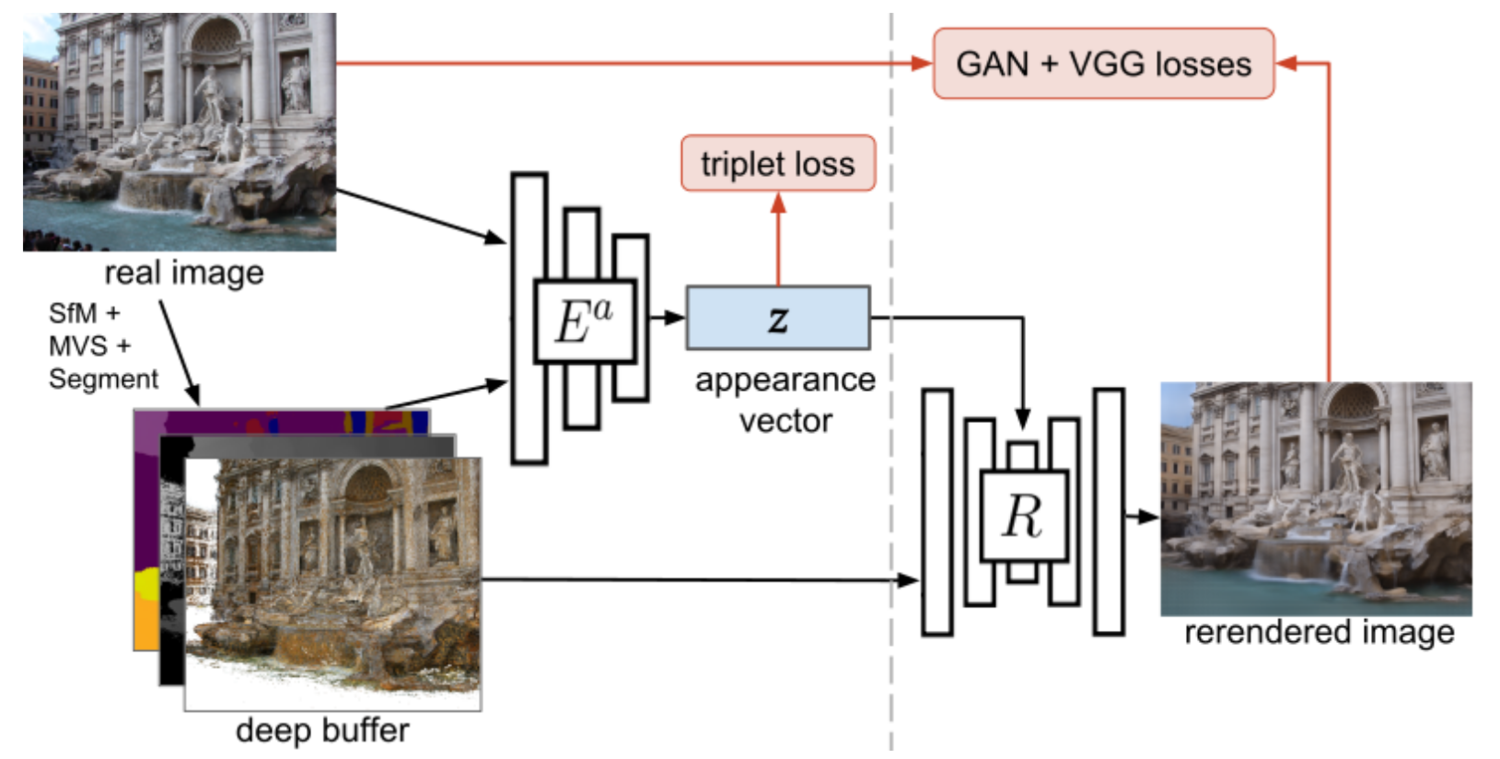
\includegraphics[width=.9\textwidth]{../graphics/nriw.png}
    \caption[NRIW model training]{Both neural networks are trained in a staged approach
    that pre-trains the appearance encoder~$E^a$ using a triplet loss, subsequently the
    rerenderer~$R$ is trained with standard reconstruction and GAN losses (right), and
    finally, fine-tuned together with~$E^a$. Taken from~\citet{NRIW}.}\label{fig:nriw}
\end{figure}

The training process works as follows---to stabilize the joint training of~$R$ and~$E^a$, and improve
the model expressiveness, pre-training the appearance encoder~$E^a$ on a proxy task is first performed.
In a staging manner, rendering network~$R$ is then trained using fixed~$E^a$ weights, allowing~$R$ to
find the correlations between output images and the embedding produced by the proxy task~$E^a$ training.
Finally, both networks are jointly fine-tuned.

The appearance pre-training works on a proxy task that optimizes
embeddings of the input images in the appearance latent space based on a suitable distance metric. Similar images under the metric should also have similar embeddings. The metric itself should ignore viewport as appearance is independent of it.
For that, authors use neural style-transfer triplet loss---for each image~$I_i$, sets of~$k$ closest and
farthest neighboring images with respect to the metric below are found. From those, one positive~$I_p$
and one negative~$I_n$ image is sampled, respectively. The loss then is:

$$\mathcal{L}(I_i, I_p, I_n) = \sum_j \mathrm{max}\left(\lVert g_i^j-g_p^j\rVert^2 - \lVert g_i^j-g_n^j\rVert^2 + \alpha, 0\right)\,,$$

where~$g_i^j$ is the Gram matrix of activations at the~$j$-th layer of a VGG network of image~$I_i$,
and~$\alpha$ is a separation margin.

Lastly, semantic conditioning performed by concatenating a semantic labeling~$S_i$ of
image~$I_i$ to the deep buffer~$B_i$ is used to account for transient objects. The authors argue that
it discourages the appearance encoder network from encoding variations caused by the location of
transient objects in the appearance latent space or associating such objects with specific viewports.

\section{Surface Splatting}

Surface splatting, presented by~\citet{SurfaceSplatting}, is an efficient technique for rendering high-quality
images of point clouds (point-sampled surfaces), supported by rigorous mathematical analysis around
resampling. In contrast to ray-tracing, it is a forward-projection approach that uses z-buffer to
resolve visibility. It can avoid aliasing artifacts brought alongside discretizing otherwise
continuous space by a screen space formulation of the Elliptical Weighted Average (EWA) filter for
irregularly spaced point samples without global texture parameterization.

It can be seen as a resampling process in signal processing~\citep{PointRendering}, effectively the method
strives to reconstruct initially hole-free surfaces sampled in the form of a point cloud. To do so, the method
uses a combination of an object-space reconstruction filter and a screen-space filter for each point primitive.
The mathematical object-space reconstruction filter (\emph{footprint function}~$\rho_i(\mathbf{x})$ of a point~$\mathbf{x}$)
resembles typically an elliptical disk, a so-called splat whose position, orientation, and axes are usually
chosen to provide a good approximation to the underlying source geometry. After a perspective projection of all splats
to the screen space, the EWA filter mentioned above is used to avoid frequencies higher than the Nyquist frequency
of the pixel sampling grid, and all contributions from the overlapping splats are combined.

\SaveVerb{term}|GL_POINTS|
\begin{figure}
    \centering
    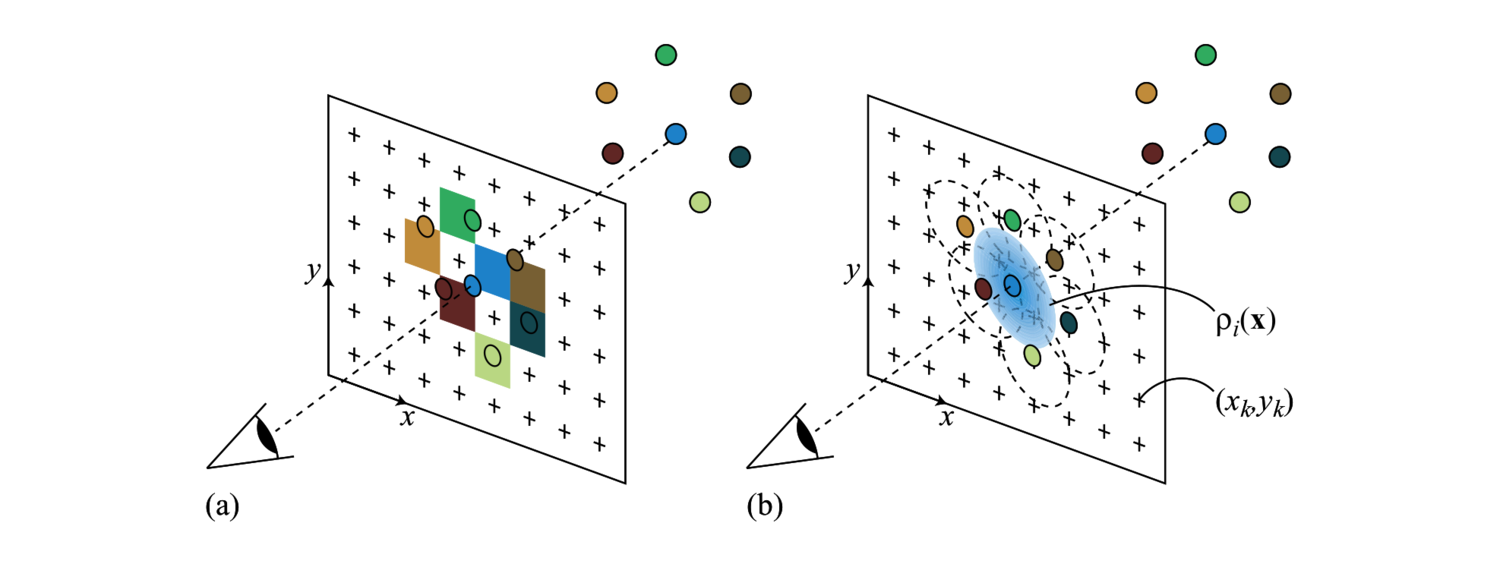
\includegraphics[width=.9\textwidth]{../graphics/splatting_principle.png}
    \caption[Surface splatting compared to simple projection]{Point rendering
    by surface splatting compared to a naive approach that is used, for instance,
    by \protect\UseVerb{term} OpenGL primitive. (a) Naive forward projection and rendering of point samples
    assigning the projected point's color to the closest pixel in the screen space. (b) By splatting footprint
    functions, each pixel gets color decided upon a combination of contributions scree-space neighboring points.
    Taken from~\citet{PointRendering}.}\label{fig:splatting_principle}
\end{figure}

The basic idea of splatting compared to a naive approach is shown in~\cref{fig:splatting_principle}.
The naive method does not work generally as it leads to holes in reconstructed surfaces in the rendered image
if the surface is not sampled with sufficient frequency. Also, another disadvantage happens when more than
one point gets projected to the same closest pixel---then the rendering result depends on the order in
which the points are processed. Surface splatting alleviates the problems by distributing the color of
each projected point among more neighboring screen-space pixels with a suitable footprint function.
The desirable footprint function is usually smooth, decays quickly with increasing
distance from the projected center, and has local support as indicated by the ellipses in~\cref{fig:splatting_principle}.

For a single channel of a possible multiple-channel (taken independently) image, image function~$\phi(x, y)$
taking a pixel position and returning color could be defined according to previous thoughts as

\begin{equation}\label{eq:simple_splatting}
\phi(x, y) = \sum_i c_i\rho_i(x, y)\,,
\end{equation}
where the sum is carried over the indices of all points~$\{\mathbf{p}_i\}$ of the surface, $\rho_i$ are individual
footprint functions, and~$c_i$ are channel color values of a given point.

The definition~\cref{eq:simple_splatting} has an issue with reproducing surfaces with constant color and thus can
lead to visible artifacts. Also, footprint functions are truncated to finite support. Both leads to the below presented
normalized image function used by surface splatting

\begin{equation}\label{eq:normalized_splatting}
\phi(x, y) = \sum_i c_i\frac{\rho_i(x, y)}{\sum_k \rho_k(x, y)}\,.
\end{equation}
The image function defined by~\cref{eq:normalized_splatting} leads to a two-pass algorithm for
rendering~\cref{algo:splatting}. In the first pass, all points are iterated over and their splat
footprints~$\rho_i$ and channel values~$c_i$ are computed. The footprint functions are evaluated at each pixel, or
rasterized, and their contributions are accumulated in a buffer. At each pixel~$(x, y)$,
the buffer stores the sum of the weighted contributions from the right side of~\cref{eq:simple_splatting},
normalization factor sum from the denominator of~\cref{eq:normalized_splatting} and the depth for z-buffering.
In the second pass, all pixels are processed by normalization of the accumulated contributions by the accumulated
normalization factor.

\begin{algorithm}[t]
	\caption{Pseudocode of the splatting algorithm.}\label{algo:splatting}
	\begin{algorithmic}[1]
		\Procedure{splat\_rendering}{p[], c[], w[], z[]}
			\For{all points i \textbf{in} p[]}
					\State rho\_i $\gets$ footprint(p\_i)
					\State c\_i $\gets$ shade(p\_i)
                        \State rasterize(rho\_i, c\_i, c[], w[], z[])
			\EndFor
			\For{all points [x, y]}
                        \State c[x, y] /= w[x, y]
			\EndFor
		\EndProcedure
	\end{algorithmic}
\end{algorithm}

How usable footprint functions are found and look is beyond the scope of this work as it requires
signal-processing theory, Gaussian functions, and the Nyquist theorem. We utilize
a GPU implementation by Sebastian Lipponer\footnotei{.}{\url{https://github.com/sebastianlipponer/surface_splatting}}

\section{Ray Marching with Signed Distance Fields}

This method is an example of a ray-casting approach, in which a finite series of steps along
a ray cast from a camera through a pixel is undertaken, until the ray hits an object or
the maximum number of permitted steps is exceeded. This very simple idea is fundamental in
computer graphics and dates back to works like~\citet{RayMarching, Hypertexture}. Building
on the idea, many effects, such as lights, shadows, and transparency, can be incorporated, to
name a few~\citep{RealTimeRendering}. This thesis implements a variant of the method using
\emph{signed distance functions} (SDF).

In a given scene consisting of solid bodies, a \emph{signed distance function} is a scalar
function~$S(P)$ defined at every point~$P$ in a (2D or 3D) space, such that

\begin{equation}\label{eq:sdf_def}
\begin{array}{ll}
S(P) = 0 & \text{when it is on the surface of a body,}\\
S(P) > 0 & \text{when it is inside any body,}\\
S(P) < 0 & \text{when it is outside all bodies~\citep{SDF}.}
\end{array}
\end{equation}

A \emph{scene SDF} defines the scene implicitly. An \emph{object SDF} is the SDF of a scene containing
only that one object. Object SDFs can be computed analytically for simple shapes; see
work of Inigo Quilez\footnotei{,}{\url{https://iquilezles.org/articles/distfunctions}}
or tabulated in grids, octrees, or other spatial data structures. A scene SDF can then be constructed
by combining SDFs of objects in the scene. For simple analytically-describable shapes, an
insight into how such a scene can be built may be given through Constructive
Solid Geometry (CSG), a method of creating complex geometric shapes from simple ones via boolean
operations, see the left of~\cref{fig:rm}. This process has its mirror in combining SDFs; see code example in~\cref{code:sdfs}.
As an example, an SDF for the simplest 3D object, a sphere positioned at the origin and with a defined radius,
is \verb|SDF_sphere(vec3 pos) -> length(pos) - RADIUS|. In general, SDF does not need to be based on Euclidean distance
and may be exact or approximate. The only theoretical requirement is~\cref{eq:sdf_def} and from a practicality perspective,
evaluation of such a function should be reasonably quick.
The algorithm utilizing a scene SDF is outlined in~\cref{algo:marching}. The visual representation of
the simplest form of the algorithm proceeding along a ray is to be found in the right of~\cref{fig:rm}.

\begin{lstlisting}[language=Python,caption=Code example showing how SDFs of simpler object can be combined together to gradually build a scene SDF., label=code:sdfs]
def SDFintersect(obj1_SDF, obj2_SDF):
    return max(obj1_SDF, obj2_SDF)

def SDFunion(obj1_SDF, obj2_SDF):
    return min(obj1_SDF, obj2_SDF)

def SDFdifference(obj1_SDF, obj2_SDF):
    return max(obj1_SDF, -obj2_SDF)
\end{lstlisting}

\begin{figure}
	\centering
	\begin{subfigure}{.5\textwidth}
		\centering
		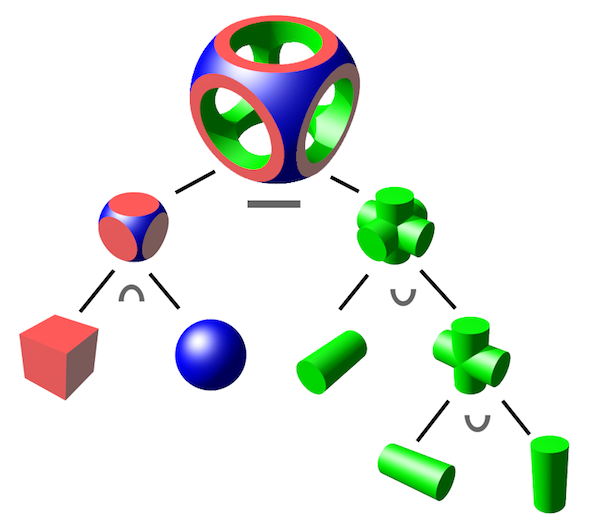
\includegraphics[width=.9\textwidth]{../graphics/csg.png}\label{fig:csg}
	\end{subfigure}%
	\begin{subfigure}{.5\textwidth}
		\centering
		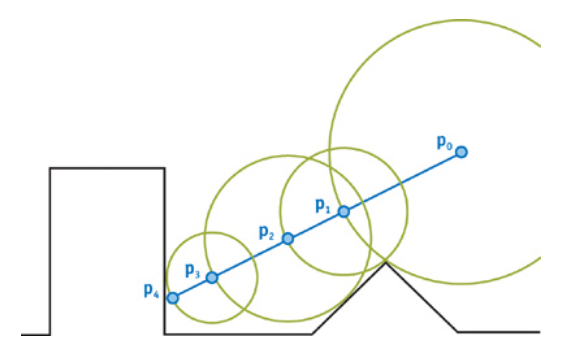
\includegraphics[width=.9\textwidth]{../graphics/marching.png} \label{fig:marching}
	\end{subfigure}
	\caption[Ray Marching and Constructive Solid Geometry]{Left: CSG is
        built upon three primitive operations: intersection ($\cap$),
        union ($\cup$), and difference ($-$).
        Taken from~\url{https://en.wikipedia.org/wiki/Constructive_solid_geometry}. Right: Demonstration
        of ray marching where at each step algorithm proceeds along given ray by a distance to the
        closest surface as it is a safe way how to find a hit, based on some threshold distance.
        Taken from~\url{https://jamie-wong.com/2016/07/15/ray-marching-signed-distance-functions/}.} \label{fig:rm}
\end{figure}

In this thesis, we utilize scene representation relying on translated sphere SDFs with radii precomputed beforehand
to be dependent on the distance to the closest neighbor for a given point primitive. Scene SDF for such a
scene would be then a minimum of all point SDFs in the scene (following again~\cref{code:sdfs}). This naive
declaration is not scalable to millions of points a scene produced by a LiDAR or SfM may contain, even though
only the simplest point primitives are used for the rendering process. To increase significantly rendering performance
with sufficient reality reproduction capabilities, we take advantage of a spatial 3D KD-tree~\citep{KDTree}
implemented in NVIDIA CUDA\footnote{\url{https://developer.nvidia.com/cuda-toolkit}} toolkit that can quickly
return the closest point for a given location. Since the exact sphere SDF contains its radius and KD-tree built
on top of the source point cloud returns the distance to the sphere center (point) itself, not the distance to the sphere's surface,
we take~$N$ closest points, instead of just one, compute exact SDF for those with their respective radii, and then take the point
at the minimal distance determined. The same KD-tree is pre-build once at the start of the rendering process and
is also used for radii computation instead of computing those exhaustively.


\begin{algorithm}[t]
    \caption{Pseudocode of the ray marching with SDF.}\label{algo:marching}
    \begin{algorithmic}[1]
        \Procedure{ray\_march}{ray\_origin, ray\_direction}
            \State dist $\gets$ 0
            \For{i \textbf{in} range(MAX\_STEPS)}\Comment{Hyperparameter to stop traversal}
                \State current\_pos $\gets$ ray\_origin $+$ dist $*$ ray\_direction
                \State closest $\gets$ SDFscene(current\_pos)
                \If{closest.dist $<$ MIN\_HIT\_DIST}\Comment{Float comparison}
                    \State \textbf{return} closest.color
                \EndIf
                \If{dist $>$ MAX\_DIST}\Comment{No hit along the ray}
                    \State \textbf{return} BACKGROUND\_COLOR
                \EndIf
                \State dist $\gets$ dist $+$ closest.dist
            \EndFor
        \EndProcedure
    \end{algorithmic}
\end{algorithm}

\chapter{Camera Pose Verification}

In the chapter, datasets, their transformations, and experiments performed upon them with
the introduced methods' implementations are all presented. We use the generalized InLoc
pipeline with a modified pose verification step. The synthesized image leveraged for
pixel-wise computation of similarity with the given query image is swapped with views
generated by renderers presented in the preceding chapter, depicting the scene's point
cloud from estimated query positions. Apart from how the synthesized image is generated,
the rest of the verification process is then performed according to the original article,
using namely RootSIFT descriptors.\\

While discussing concrete details of datasets' definitions and algorithms' inputs, more
technical aspects are taken into account---among them, of utmost importance are
conventions used by coordinate systems in which points of explicit scene representations
are expressed/expected to be and by matrices related to cameras taking database images.
These pose a crucial difference between what a dataset provides, or localization pipeline
expects and must be addressed by implementation to obtain valid localization results.

\begin{figure}
    \centering
    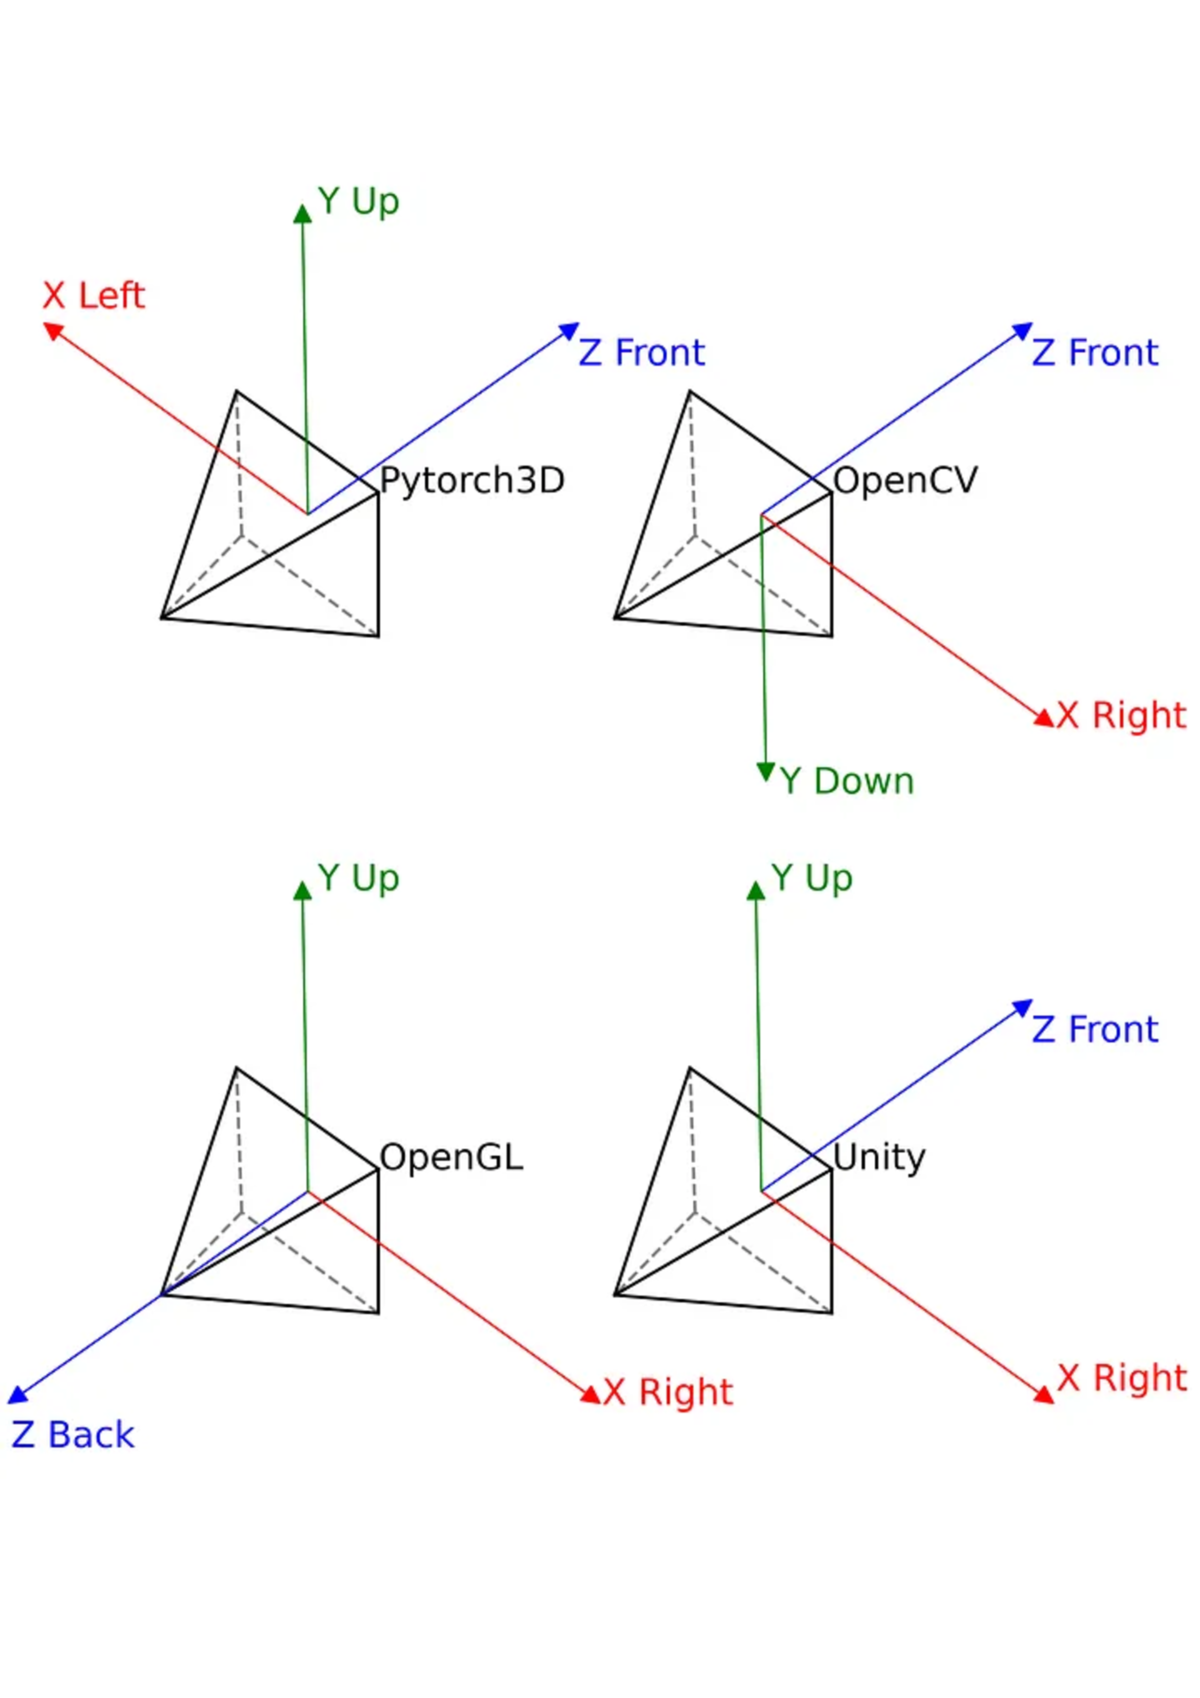
\includegraphics[width=.7\textwidth]{../graphics/cs_conventions.png}
    \caption[Examples of various camera\,/\,coordinate frame conventions]{
    Examples of various camera\,/\,coordinate frame conventions used by
    common programmatic tools in fields dealing with computer graphics.
    Taken from~\url{https://medium.com/check-visit-computer-vision/converting-camera-poses-from-opencv-to-opengl-can-be-easy-27ff6c413bdb}.}\label{fig:cs_conventions}
\end{figure}

Coordinate system conventions address the decision of assigning positive directions,
labels, and meanings in the human sense (up, right, forward) to the orthogonal frame of a
3D space, because without that an oriented triplet representing a point is meaningless.
These conventions can be arbitrary depending on whether they come from computer vision,
rendering, or another field. Examples of such conventions, linked to standard computer
graphics libraries/tools that use/expect them, can be found in~\cref{fig:cs_conventions}.
In this thesis, computer vision and rendering conventions are used. In the
figure~\cref{fig:cs_conventions}, these are found alongside OpenCV and OpenGL labels,
respectively. Even though both are right-handed, they understand x, y, and z point
components differently.  In rendering, the positive x-axis points to the right, the
positive y-axis up, and the positive z-axis towards a viewer looking at the coordinate
system frame. In computer vision, the positive x-axis points to the right, the positive
y-axis to the bottom, and the z-axis away from the same viewer as before. Transformation
matrices operating over both notations are thus related by inverting the y and z axes
columns. As an example, since a camera in rendering is typically placed along z-xis,
failing to take this relation into account when displaying a 3D model defined in computer
vision notation in a visualization tool that uses rendering notation results in rendering
half-space \uv{away} from the model. For instance, in the case of other notations used by
a produced model, a rendered view can be somewhat unexpectedly rotated.

Matrix conventions in the context of the thesis are related to terms coming from the
graphics pipeline---\emph{world space} and \emph{view space}. In the case of datasets
described below, world space is a space of the whole scene representation with the origin
and orientation of the coordinate frame chosen arbitrarily in relation to the scene.  The
randomness in the coordinate frame placement is especially true in the case of
SfM-generated scene models, where the algorithm decides these parameters.  When preparing
a model manually, e.g., in the game industry, the frame is typically artificially placed
meaningfully concerning the model produced, e.g., along the outer edges of a cube model.
View space is a space of a camera looking at a portion of the scene---origin is the center
of the camera with the coordinate frame oriented in a specific way alongside the optical
axis of the camera depending on the exact graphics pipeline/tool used.
Visualisation~\cref{fig:cs_conventions} can be used here as well---the square pyramids
depict view frustums of virtual cameras, with the z-axes being their optical axes.

Provided both spaces are same-handed, the matrix inverse relates transformations between
them. In homogeneous coordinates, both transformations are represented by $4\times4$
matrices, and the implementation must correctly distinguish between the actual meaning of
these 16~real numbers, including how the matrix is stored on the disk. We refer to them as
the \emph{view matrix} transforming from world to view space and \emph{camera pose}
representing the opposite, inverse transformation.

\section{Datasets}

Several image collections were used for measuring localization performance, both indoors
and outdoors. To ensure continuity and comparability with previous works of~\citet{InLoc,
Bastien}, we utilize the open-source InLoc Dataset presented in the original Inloc
paper~\citep{InLoc}. Another closed-source, indoor dataset is a 3D scanner-generated
digital twin of a SIEMENS manufacturing facility that is targeted by several use cases of
the Industry \& Construction 4.0 Solutions project called ARTwin, financially supported by
the European Union's Horizon 2020 research and innovation program. Finally, an outdoor
dataset is covered by the inclusion of the open-source Phototourism dataset from the Image
Matching Challenge
2021\footnotei{.}{\url{https://www.cs.ubc.ca/research/image-matching-challenge/2021}}

\subsection{InLoc Dataset}

The dataset consists of a database of Faro 3D scanner-generated RGBD scans that are
geometrically registered to the floor plan of two buildings of Washington University in
St. Louis. The test set is a composition of RGB photos taken by a hand-held device (an
iPhone).

277 RGBD panoramic images have ground truth poses in the global coordinate system spanning
across the floor plan. Each RGBD panoramic scan is a point cloud (\emph{scan}) having
roughly 40~million colored points. The final dataset is generated by obtaining
36~perspective RGBD images from each panorama by extracting standard perspective views
($60^{\circ}$~FoV) with a sampling stride of $30^{\circ}$ in yaw and $\pm30^{\circ}$ in
pitch directions, resulting in cca 10~thousand perspective images in total, examples are
in~\cref{fig:inloc_dataset}. This dataset contains all troublesome elements for indoor
localization, namely repetitive patterns (such as stairs and pillars), global and local
similarities (doors, windows), furniture changing positions in the test set, people moving
across the scene, and textureless, highly symmetric areas (walls, floors, corridors,
classrooms, open spaces).

The original query set consists of 356~photos taken by an iPhone~7 at various lighting
conditions within a day, capturing a variety of occluders and layouts (people, furniture),
also covering only a subset of the floor plan data, with the rest playing the role of
confuser at search time. Ground truth poses for the test set are not publicly accessible,
and evaluation can be done only indirectly via submission to the Visual
Localization\footnote{\url{https://www.visuallocalization.net}} page.

The structure of the dataset's database folder is as follows---\verb|scans/<FLOOR>|
folders, where \verb|FLOOR| is one of DUC1, DUC2, CSE3, CSE4, and CSE5, representing five
floors of the two mentioned buildings (CSE, DUC), contain files named
\verb|<NAME_WITH_SCAN_NUMBER>.ptx.mat| storing RGB and XYZ information of scanned points
in Matlab file format. Every floor has its specific number of scans, uniquely numbered
within a building. Final dataset's perspective views are stored in folders
\verb|cutouts/<FLOOR>/<SCAN_NUMBER>| containing JPG perspective RGB images of size
$1600\times1200$ pixels and MAT files containing bundled RGB perspective image (RGBcut)
and the respective scan points (XYZcut). Files
\verb|alignments/<FLOOR>/transformations/<NAME_WITH_SCAN_NUMBER>.txt| contain $4\times4$
transformation matrices that convert 3D homogeneous points in original .ptx.mat files to
the global coordinate system of the floor plan.

The dataset's query folder contains one subfolder named \verb|iphone7| with the query set
of photos taken by the iPhone camera. Photos are stored as JPG files of size
$4032\times3024$ or $3024\times4032$ pixels, so both landscape and vertical acquisition
modes were used. As the database is landscape, for InLoc algorithm processing, all images
are made landscape, and the ones where the view was changed by rotation are remembered.
Notably, even though sharing the same aspect ratio with the database after such operation,
which InLoc localization pipeline can handle, resizing to the matching dimensions is also
used to speed up the localization performance.

\begin{figure}
    \centering
    \begin{subfigure}{.5\textwidth}
        \centering
        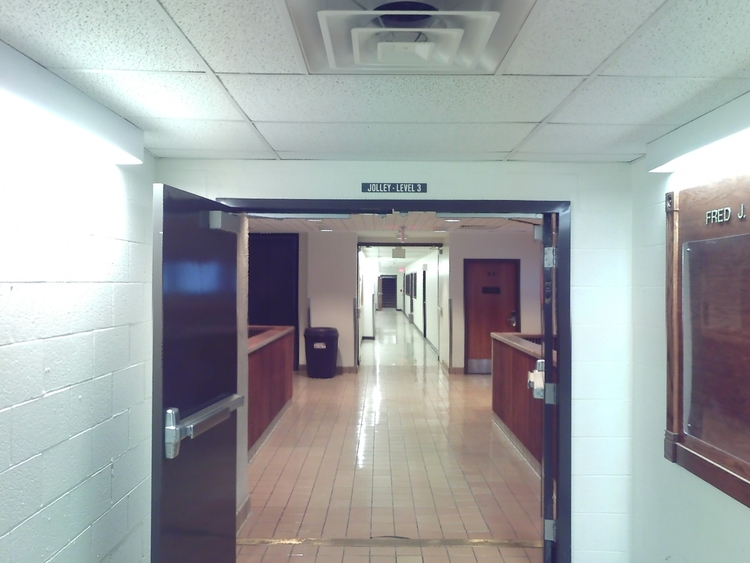
\includegraphics[width=.9\textwidth]{../graphics/cse_cutout_000_90_0.jpg}
    \end{subfigure}%
    \begin{subfigure}{.5\textwidth}
        \centering
        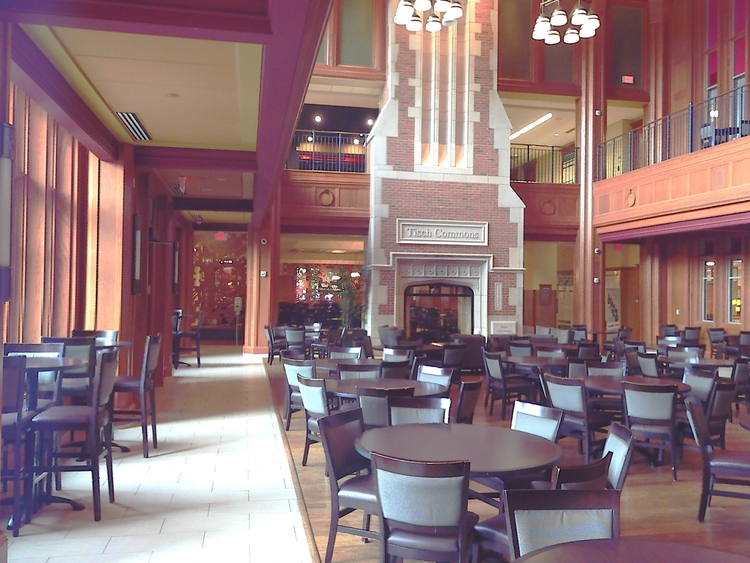
\includegraphics[width=.9\textwidth]{../graphics/DUC_cutout_003_0_0.jpg}
    \end{subfigure}
    \caption[Samples from InLoc dataset database images]{Samples from InLoc dataset database images.}\label{fig:inloc_dataset}
\end{figure}

\subsection{ARTwin Dataset}

The dataset consists of registered $360^{\circ}$ RGB panoramic images across two halls of
a SIEMENS manufacturing facility together with point clouds for both produced by merging
3D data from a NavVis 3D scanner.

Over the two halls, 29 and 53~panoramic images were obtained. The final dataset used in
this thesis contains roughly 4~thousand processed images and it is generated in accordance
with InLoc Dataset except for a difference in the necessity to remap
$360^{\circ}$~spherical panorama to 2D~surface again, examples are
in~\cref{fig:artwin_dataset}. Hall point clouds are not matched to a common coordinate
system as they overlap when displayed together, so for localization disambiguation one
hall is lifted along the z-axis.

The raw dataset contains all the intermediate files, photos and logs from the acquiring
process together with processed and merged results mentioned above. The structure of the
relevant processed data is \verb|proc/<HALL_ID>|, IDs of the halls are
\verb|2019-09-28_08.31.29| and \verb|2019-09-28_16.11.53|. Within each of these folders,
there is processed point cloud \verb|<HALL_ID>.ply| and \verb|pano| folder with JPG
panoramic scans alongside \verb|pano-poses.csv|. Poses are in the form of 3D scanner
position and orientation quaternion per panoramic scan.

\SaveVerb{hall53}|2019-09-28_16.11.53|
\SaveVerb{hall29}|2019-09-28_08.31.29|
\begin{figure}
	\centering
	\begin{subfigure}{.5\textwidth}
		\centering
		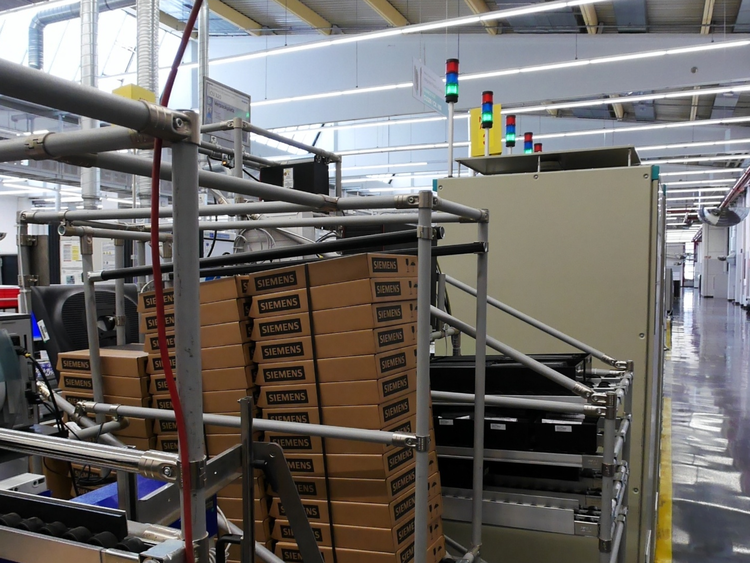
\includegraphics[width=.9\textwidth]{../graphics/2019-09-28_16.11.53_00000_x0_z90_reference.png}
	\end{subfigure}%
	\begin{subfigure}{.5\textwidth}
		\centering
		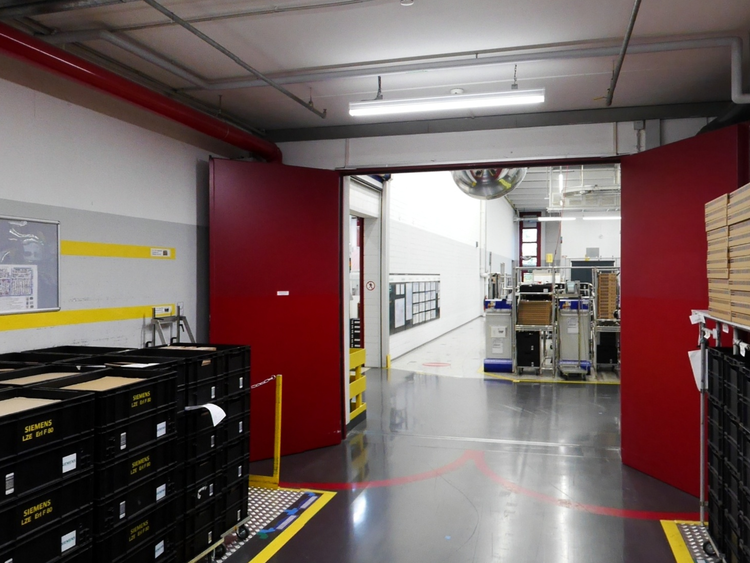
\includegraphics[width=.9\textwidth]{../graphics/2019-09-28_08.31.29_00000_x0_z60_reference.png}
	\end{subfigure}
	\caption[Sample flattened images from ARTwin dataset]{Sample
        flattened images from ARTwin dataset, on the left hall
        \protect\UseVerb{hall53} is presented, on the right
        \protect\UseVerb{hall29}.}\label{fig:artwin_dataset}
\end{figure}

\subsection{Phototourism Dataset}

The smallest datasets taken from the Image Matching Challenge (IMC) data, photo-tourism image
collections depicts several popular landmarks, collected from the Yahoo Flickr Creative
Commons 100M (YFCC) dataset. Namely, Hagia Sophia Interior, Pantheon Exterior, and Grand
Place Brussels collections were used. These datasets have around $1\,000$~photos each
coming, using the terminology from~\citet{NRIW}, \uv{from the wild} as they were taken by
many authors, at various distances and with sensor sizes varying considerably,
see~\cref{fig:imc_dataset}.

\begin{figure}
	\centering
	\begin{subfigure}{.5\textwidth}
		\centering
		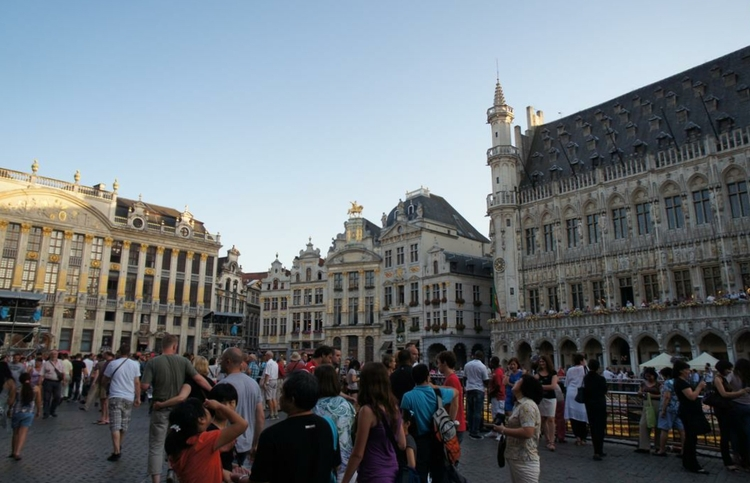
\includegraphics[width=.9\textwidth]{../graphics/grand_06498281_8296173847.jpg}
	\end{subfigure}%
	\begin{subfigure}{.5\textwidth}
		\centering
		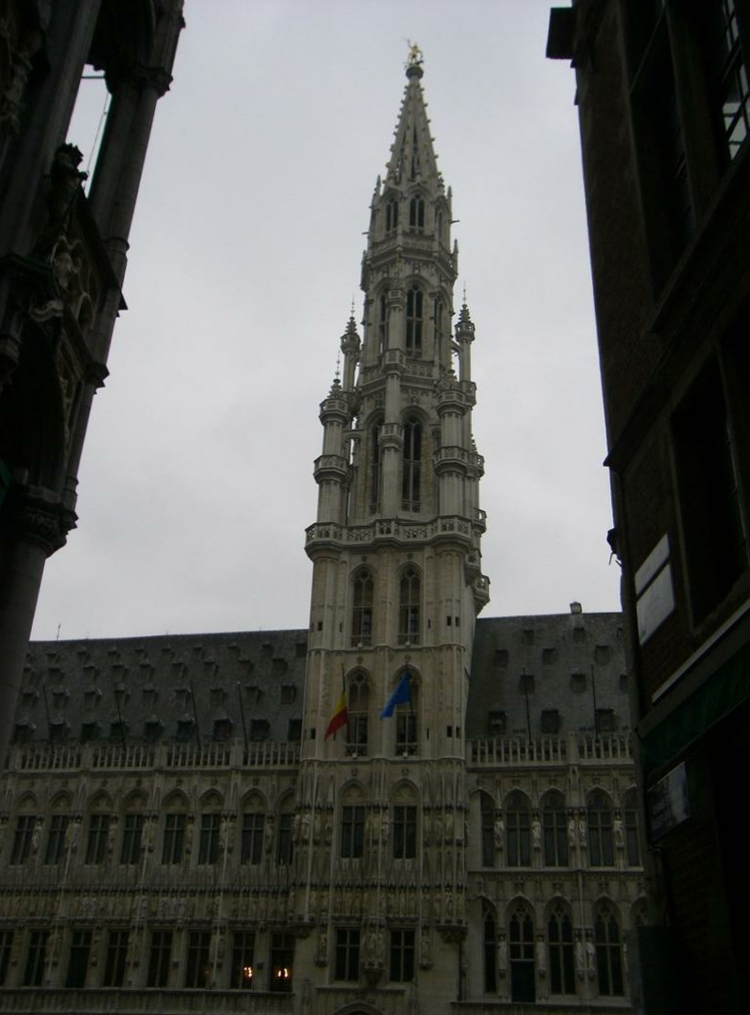
\includegraphics[width=.9\textwidth]{../graphics/grand_01352021_435013564.jpg}
	\end{subfigure}
	\begin{subfigure}{.5\textwidth}
		\centering
		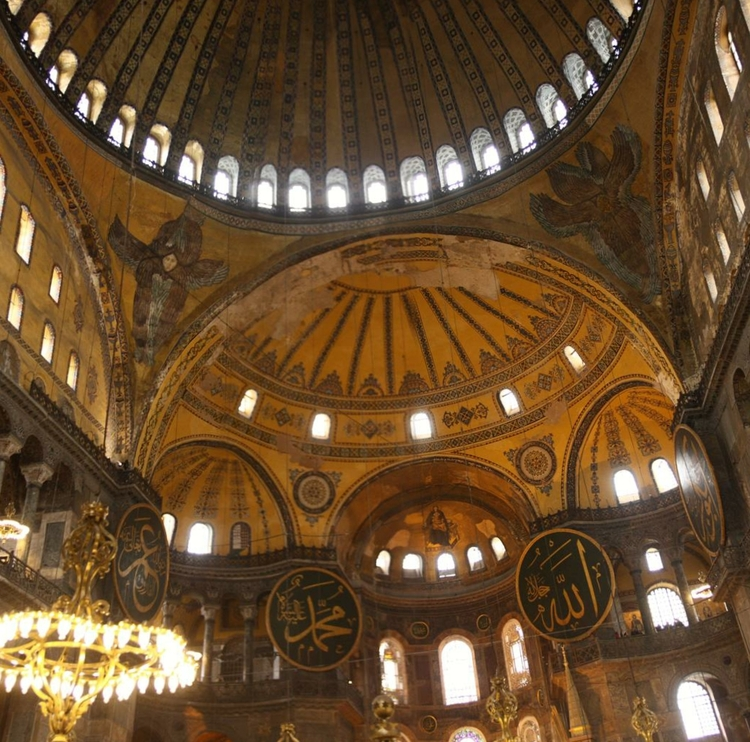
\includegraphics[width=.9\textwidth]{../graphics/hagia_04240457_5644708528.jpg}
	\end{subfigure}%
	\begin{subfigure}{.5\textwidth}
		\centering
		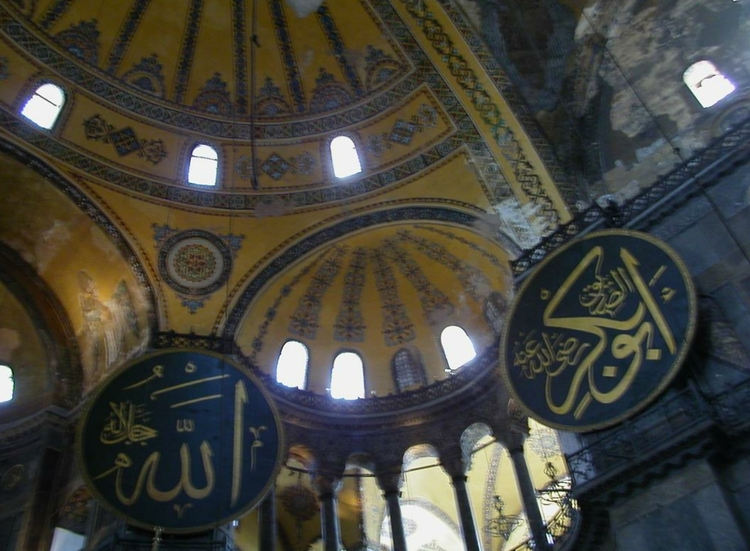
\includegraphics[width=.9\textwidth]{../graphics/hagia_01058134_62294335.jpg}
	\end{subfigure}
	\begin{subfigure}{.5\textwidth}
		\centering
		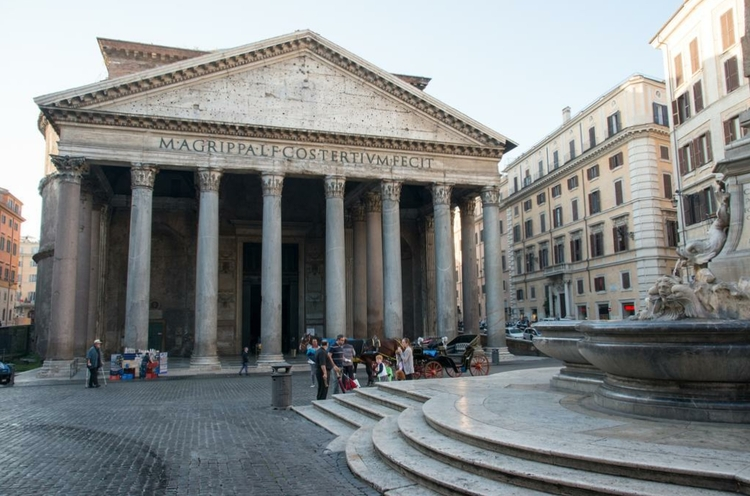
\includegraphics[width=.9\textwidth]{../graphics/pantheon_00488011_10505838106.jpg}
	\end{subfigure}%
	\begin{subfigure}{.5\textwidth}
		\centering
		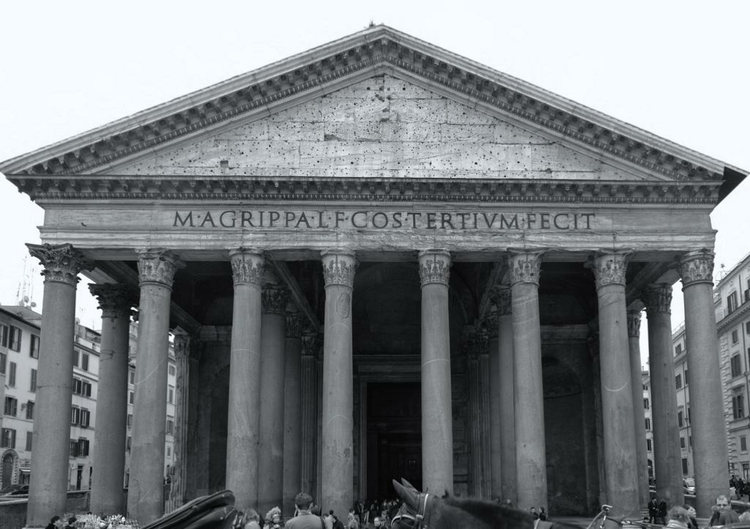
\includegraphics[width=.9\textwidth]{../graphics/pantheon_00927614_8536847775.jpg}
	\end{subfigure}
	\caption[Sample images from Phototourism dataset]{Sample images from
        Phototourism dataset taken \uv{from
        the wild}, stretching various aspect ratios, sizes, time of the day of the
        aquisition, and varying lighting conditions present in the data. In the top
        row there are images of Grand Place in Brussels, below of interior of Hagia
        Sophia Grand Mosque in Istanbul, and in the bottom of Pantheon in
        Rome.}\label{fig:imc_dataset}
\end{figure}

The dataset per given collection used in the thesis is built on top of raw images by
running COLMAP software. Structure of the COLMAP produced dataset is described in its
documentation\footnotei{.}{\url{https://colmap.github.io/format.html}} Shortly, there is
\verb|dense/sparse/cameras.bin| file with parameters of cameras capturing wild images
retrieved by SfM method implemented in COLMAP, \verb|dense/sparse/images.bin| file with
retrieved 3D positions and orientation quaternions of each image in a common coordinate
system of \verb|dense/fused.ply| point cloud. This point cloud is generated by SfM from
implicit scene representation contrary to the previously mentioned datasets that represent
a 3D scanner-generated approach.\\

Putting everything together---all scene point clouds for all datasets explored in the
thesis are placed in the right-handed coordinate system, though conventions of the
coordinate frames vary, described  side-by-side in~\cref{tab:model_conventions}. In order
to properly render a virtual view, related camera poses must be preprocessed accordingly.
Another side-by-side comparison of the datasets can be found in~\cref{tab:datasets}
presenting their basic statistical features.

\begin{table}
\caption[Comparison of conventions and notations found in scene representations of all
datasets explored in the thesis]{Comparison of conventions and notations found
in scene representations of all datasets explored in the thesis.}
\centering
    \begin{tabular}{p{4cm} p{4cm} p{4cm}}
    \toprule
    ARTwin & InLoc Dataset & IMC \\
    \midrule
    Right-handed coordinate system, scans use convention where in order to be
    rendered by an OpenGL camera to match database images, in sequence, x-y and y-z axes
    must be switched. There is no notion of global CS where both hall point clouds can be
    placed, so an artificial translation along z-axis is performed on the hall labeled 53
    for localization disambiguation. & Right-handed coordinate system, scans use
    convention where in order to be rendered by an OpenGL camera to match database images,
    in sequence, x-y and y-z axes must be switched. For each scan, a transformation from
    local to the defined global CS is known. & Right-handed coordinate system, model in computer vision (CV)
    notation. To render properly by an OpenGL camera to match database images, y and z
    axes must be inverted.  COLMAP-generated per-view matrices are view matrices.\\
    \bottomrule
    \end{tabular}
\label{tab:model_conventions}
\end{table}

\begin{table}
\caption[Comparison of various features of all datasets used in the thesis]{
Comparison of various features of all datasets used in the thesis.
InLoc test set specified here is generated from the dataset so that we have the ground
truth poses, otherwise the online evaluation tool would need to be used. Number of points
in a scan refers to the mean of points count for iInLoc and ARTwin datasets, and to the
number of points in the whole scene model for the rest. Dimensions are specified in
thousands of pixels and for Phototourism datasets it is not applicable as source photos
have various dimensions.}
\centering
    \begin{tabular}{l c c c c c}
    \toprule
     & InLoc & ARTwin & Hagia Sophia & Pantheon & Grand Place\\
    \midrule
    Train Size  &	7\,977 	& 2\,423    & 670 & 1\,078  & 821\\
    Val Size    &	1\,995	& 379       & 167 & 269     & 205\\
    Test Size   &	356	    & 150       & 50  & 50		& 50\\
    Scan Points	&   40M     & 27M       & 5M  & 5M		& 4M\\
    Dims [k pix]& 1.6x1.2	& 1.6x1.2	& -   & -		& -\\
    \bottomrule
    \end{tabular}
\label{tab:datasets}
\end{table}

\section{Implementation}

For purposes of the thesis, several code projects are leveraged, either built from the
ground up by the author or based on top of the previous work of others.  Localization
InLoc framework is based on the work of the article author Hajime Taira and further
enhancements done by Pavel Lucivnak and Bastien Dechamps spread across several code
repositories. From renderers, for Neural Rerendering in the Wild, the authors'
implementation with surrounding scripts written by Bastien Dechamps is used as the base of
further work. For surface splatting, the great work of Sebastian Lipponer, with some
tweaks, is leveraged. Finally, the ray marching renderer based on OpenGL is entirely the
author's work.

Aside from the localization algorithm and renderers, scripts transforming dataset formats,
described in~\cref{tab:model_conventions}, into notations and conventions used by the InLoc
pipeline and renderers themselves as described in~\cref{tab:agorithm_conventions}
are also added; for more information, see below.\\

To be runnable in CIIRC computational cluster environment, which distributes jobs
submitted by users by Slurm\footnote{\url{https://www.schedmd.com}}, batch job shell
scripts are written. Slurm is an open-source, fault-tolerant, and highly scalable cluster
management and job scheduling system for clusters of Linux-running machines. Slurm
requires the batch job scripts to specify memory, CPU, and GPU requirements for
encompassed computation. Specifying these in the code results in less time for experiment
reproduction; it can also be immediately seen whether one has enough resources to run it
in the first place. These bounds vary greatly for algorithms and models utilized in this
thesis, from a few GB of RAM to almost 400 GB for InLoc processing the InLoc dataset, zero
to eight GPUs for NRIW training, and typically a few CPU cores.\\

Alongside these shell scripts, an attempt to have a reproducible experimental pipeline was
made using \emph{Docker}/\emph{Singularity} and \emph{DVC}.

Docker\footnote{\url{https://www.docker.com}} is an industry-grade platform allowing to
build, test, and deploy applications quickly and robustly. Docker is an example of
container-based virtualization, where a container is a running \uv{image} that packs
everything the software needs for running, including libraries, system tools, code, and
runtime. This approach is suitable for computational cluster environments as the code can
be executed without relying on cluster administrators to install necessary packages
globally for all users, which often leads to software version collisions.
Containerization is a more lightweight virtualization technique compared to classical
virtual machines resulting in quick startup times, lower memory requirements overhead, and
a more user-friendly working experience suitable for both development and
productionalisation. Technically, this is enabled by sharing underlying OS kernel by all
running containers, contrary to virtual machines that are ran on bare metal with the
so-called hypervisor, emulating their own OS kernels separated from other virtual machines
running on the same hardware. To be more specific, the thesis relies on GPU-based
computations; to be able to run GPU workloads in a container, there is an exception to the
mentioned advantage of container-based virtualization to avoiding cluster administrators
globally changing the cluster---suitable GPU drivers must be installed. Especially for all
the renderers described to be able to use off-screen headless rendering (rendering to
textures and saving them without displaying them on a monitor) on NVIDIA GPU cards used by
the CIIRC computational cluster, a driver with bug-less EGL\footnote{EGL is an interface
between Khronos rendering APIs such as OpenGL ES or OpenVG and the underlying native
platform window system, \url{https://www.khronos.org/egl}.} support must be used, which is
something not every driver version satisfies. CUDA and OpenGL libraries are then owned by
each container, communicating with the shared driver on the operating system level.

Singularity\footnote{\url{https://sylabs.io}} is a containerization platform similar to
Docker, with one notable exception leading to the adoption of the tool by computational
cluster administrators (including CIIRC's) instead of the otherwise industry-leading and
widely used Docker---it does not require administrative privileges from its users. For
this thesis, descriptions of Docker images to be built are written where applicable. Once
built, images are transformed into Singularity variants runnable on the cluster. This
functionality is supported natively by \verb|singularity| binary as it is a common
use-case for the tool.

Data Version Control (DVC\footnote{\url{https://dvc.org}}) should help traceable and
reproducible science by leveraging the Git version system to also version data,
intermediate results, tie them with the exact code that produced them and thus track all
ideas and experiments. It also can manage workflows which is valuable for defining
reproducible data pipelines. The advantages of this tool are simplicity as it uses
Git---which is a standard tool in code development---and workflow management is done
through simple shell scripting that is well suited for the Slurm environment with running
various Singularity containers as scheduled jobs. Though the idea is promising in the
recent growth of Machine Learning Operations (MLOps), the tool proved unsuitable when used
for datasets consisting of an enormous number of smaller files which is often the case in
computer vision. DVC uses hashes to check consistency and the necessity to recompute some
steps in a workflow, so it may take many hours to run even elementary transformations.
The overhead of these hash computations is considerable, leading to the decision not to
use DVC after all.

\subsection{InLoc localization pipeline} \label{subsec:inloc}

The implementation of the
pipeline\footnote{\url{https://github.com/Auratons/inlocciirc_demo}} is based on the
Matlab sources written by the article's author\footnotei{.}{\url{https://github.com/HajimeTaira/InLoc_demo}} The
source code is unified for better readability and verifiability; it is also generalized,
as the original implementation targets specifically the InLoc
dataset\footnotei{,}{\url{https://github.com/HajimeTaira/InLoc_dataset}}. Furthermore, as
the original code lacks computation of scores and evaluation for a general dataset, the
proposed approach of Pavel Lucivnak for the former is leveraged and further
developed\footnotei{,}{\url{https://github.com/lucivpav/InLocCIIRC_demo}}
\footnote{\url{https://github.com/lucivpav/InLocCIIRC_dataset}}

The outline of the implementation is depicted by~\cref{fig:inloc_pathway}.  Cutouts for a
dataset is a folder structure containing 3~files per database (DB) image---pose file, the image
itself, and a so-called \uv{XYZcut}. The cut is a $\text{M}\times\text{N}\times3$ array
with XYZ coordinates of a surface that would be hit first by a ray cast from the center of
the camera that took the DB image of size $\text{M}\times\text{N}$ (ignoring color
dimension) through given pixel. Computation of the cuts is not part of the source InLoc
pipeline implementation, so one method of getting the cut from a particular
renderer-generated  depth map and known camera parameters is
implemented\footnotei{.}{\url{https://github.com/Auratons/inlocciirc_dataset}}
The InLoc dataset contains default XYZCuts. However, as mentioned, there is no generation
script enclosed. The method implemented in the thesis uses depth maps to reproject from 2D
to 3D space. Since these depend on the renderer, all XYZCut are recomputed per rendering
approach. The default cuts were checked for the depiction of the background---when the ray
does not hit anything in the given view frustum, the respective coordinate is a triplet of
NaNs. Since OpenGL-based renderers typically output zero as the depth value of these "not hit"
cases, reprojected points close to the origin of the cut are filtered.

A database and query image similarity score used later for image retrieval is computed as
cosine similarity of normalized feature vectors. The original implementation using the
matrix multiplication of query and database features stacked onto each other has immense
memory requirements depleting all resources when executed on the considerably extensive
InLoc dataset, thus some allowed linear algebra adjustments are made, lowering the
requirements to reasonable numbers.

For the image retrieval step, we use 100~closest database images to every given query
photo based on the similarity score, which is the same number of candidates as the origin
article.  For all these candidate poses, after transforming them into formats expected by
the renderers explored in the thesis, we produce candidate renders and use those in the
standard pose verification process described in~\cref{sec:inloc} based on the RootSIFT
descriptors. After reranking the candidate positions based on the image-render similarity,
10~best sorted candidates are outputted as in the original article.

Evaluation is done by comparing angular and spatial L2 distances between the candidate and
the query's true pose, if known. Specifically, for the InLoc dataset, the ground truth
poses for the query set are not publicly disclosed. Only an online evaluation tool
\url{https://www.visuallocalization.net/submission/} returning the fraction of correctly
localized queries within the distance and angular threshold can be used.

\begin{figure}
    \centering
    \begin{tikzpicture}[
    >={Triangle[scale width=0.8]}, thick, black!70,
    text=black,
    every new ->/.style={shorten >=-1pt}
]
    \matrix[row sep=10mm, column sep=8mm] {
        % Zeroth row
        \node (A) [data, fill=darkgreen!20, align=left] {DB Cutouts\\Query Images}; & & \\
        % First row
        \node (B) [process] {File Lists}; &
        \node (C) [data]    {DB\,\&\,Query Lists}; &
        \node (D) [process] {Compute Features}; \\
        % Second row
        \node (G) [data]    {DB$\times$Query Scores}; &
        \node (F) [process] {Compute Scores}; &
        \node (E) [data]    {DB\,\&\,Query Features}; \\
        % Third row
        \node (H) [process] {Image Retrieval}; &
        \node (I) [data]    {Retrieval Candidates}; &
        \node (J) [process] {Pose Estimation}; \\
        % Fourth row
        \node (AA) [data, fill=darkgreen!20] {Point Clouds}; &
        \node (L) [process, draw]            {Renderer}; & 
        \node (K) [data]                     {Candidate Poses}; \\
        % Fifth row
        & \node (M) [data]  {Candidate Renders}; &
        \node (N) [process] {Pose Verification}; \\
        % Sixth row
        \node (P) [process]  {Evaluation}; & &
        \node (O) [data, draw] {Best Query Poses}; \\
    };
    \graph [use existing nodes] {
        A -> B -> C -> D -> E -> F -> G -> H -> I -> J -> K ->["reformatted"'{font=\tiny,inner sep=2pt}] L -> M -> N -> O -> P;
        E -> J; AA -> L; K -> N;
    };
\end{tikzpicture}

    \caption[InLoc algorithm]{InLoc algorithm. The implementation
    outline uses terminology from the article. Rectangles represent file(s) on the disk,
    dark green ones denote algorithm inputs, and the rest are intermediate outputs except
    algorithm outputs with a border drawn. Blue nodes of the outline denote processing
    steps.  \uv{DB cutouts} are a database (DB) format the implementation expects.
    \uv{File Lists} step scans the database and query, storing valid found examples and
    query images into a file for further reference. The \uv{Renderer} step highlighted
    with border is the main concern of the thesis.}
    \label{fig:inloc_pathway}
\end{figure}

\subsection{Neural Rerendering in the Wild}

For the Neural Rerendering in the Wild, the original implementation is also
used\footnote{\url{https://github.com/google/neural_rerendering_in_the_wild}} without any
substantial changes, just minor technical enhancements, such as support for alpha channel
processing, etc\footnotei{.}{\url{https://github.com/Auratons/neural_rendering}}

All scripts needed on the path from a raw dataset to \uv{Aligned Dataset} and \uv{Cutouts}
in~\cref{fig:artwin_dset_pathway}, \cref{fig:imc_dset_pathway}
and~\cref{fig:inloc_dset_pathway} are also implemented in the repository. Aligned dataset
is expected as input to the NRIW training process after packing into a TFRecord, similar
to Cutouts being expected by the InLoc pipeline.

For ARTwin, spherical photos need to be unrolled to 2D with the exact sampling approach as
for the InLoc dataset, resulting in the set of reference images.  To be able to reuse
scripting written initially for the IMC raw dataset, the creation of COLMAP-like camera
and image information structure is implemented alongside unrolling in preprocess script.
For depth information used within the aligned dataset, the point cloud is rendered via the
load data script for ARTwin and IMC data and the render InLoc DB script for the remaining
dataset. These scripts utilize the Pyrender python package internally, transversely
\verb|GL_POINTS| OpenGL primitive for rendering. The approach is a common baseline with
previous works on the topic.  To generate an aligned dataset with point cloud renders
provided by other renderers, the \uv{Generate matrices} step is used, for both splatting
and marching, as they share technically the same headless rendering component mentioned
below.

The aligned dataset is a structure containing, in the simplest case, a triplet of an
image, a color render of the underlying scene representation by a renderer, and the
respective depth map. The triplet forms a deep buffer mentioned in the article.  In the
original article, the authors also use semantic masking in their deep buffers.  However,
when rendering a novel view not seen in the training data, the semantic mask cannot be
obtained from an actual photo. Authors thus train a separate segmentation network between
the partial deep frame buffers and the semantic masks Si to tackle this issue. However,
this makes the network more complex and lowers the prediction time performance.
Semantically segmenting the point cloud might be used, but following~\citet{Bastien}, the
additional complexity is avoided.

\begin{figure}
    \centering
    \begin{tikzpicture}[
    >={Triangle[scale width=0.8]}, thick, black!70,
    text=black,
    every new ->/.style={shorten >=-1pt},
]
    \matrix (m) [row sep=5mm, column sep=10mm] {
        % First row
        \node (A)       [data, text width=2.1cm, fill=darkgreen!20] {360\textdegree{} Scans\\ Poses}; & [-21mm]
        \node (B)       [process] {preprocess.m}; & [-8mm]
        \node (C)       [data]    {COLMAP Data \\ -- images \\ -- cameras}; & [-3mm]
        \node (helper1) [coordinate] {}; & [-2mm]
        \node (load)    [process] {load\textunderscore{}data.py}; \\ [-6mm]
        % Second row
        \node (F) [data, text width=2.1cm, fill=darkgreen!20] {Point Cloud}; & & & & \\
        % Third row
        & \node (poses) [data] {Camera Poses}; &
        \node (matrices) [process,align=center] {Generate matrices\\{\scriptsize ARTwin variant}}; & &
        \node (hall) [data]    {Aligned Hall}; \\
        % Fourth row
        & \node (renderers) [process] {Dockerized Renderers}; & & & \\ [2mm]
        % Fifth row
        \node (G) [process, anchor=text, xshift=-10mm] {build\textunderscore{}cutouts\textunderscore{}artwin.py}; & &
        \node (E) [data, draw] {Aligned Dataset}; & &
        \node (join) [process] {join\textunderscore{}datasets.py}; \\
        % Sixth row
        \node (H) [data, draw] {Cutouts}; & & & & \\
    };
    \graph [use existing nodes] {
        A -> B -> C -- helper1 -> load -> hall -> join -> E;
        hall -> [dashed] matrices -> [dashed] poses -> [dashed] renderers;
        E -> G;
    };
    \gettikzxy{(F.south west)}{\fx}{\fy}
    \gettikzxy{(renderers.south)}{\hx}{\hy}
    \gettikzxy{(F.south)}{\fsx}{\fsy}
    \gettikzxy{(G.north)}{\gx}{\gy}spot
    \gettikzxy{(G.south)}{\gsx}{\gsy}
    \gettikzxy{(H.north)}{\hhx}{\hhy}
    \draw [very thin, densely dash dot, black] ($ (\fx, \hy) + (-0.1, -0.15) $) rectangle ($ (load.north east) + (0.1, 0.51) $);
    \draw [very thin, densely dash dot, black] ($ (\fx, \hy) + (-0.15, -0.2) $) rectangle ($ (load.north east) + (0.05, 0.46) $);
    \draw [rounded corners] (F) -| (helper1) -- (load.west);
    \draw [->] (F) -- (\fsx, \gy);
    \draw [->] (\fsx, \gsy) -- (\fsx, \hhy);
    \draw [rounded corners, ->, dashed] (renderers) -| ($ (hall.south west) + (5mm, 0)$);
    \draw [rounded corners, ->, dashed] ($ (F.south) + (1mm, 0) $) |- (renderers);
    \node [above=of load.north, yshift=-5.5mm, font=\tiny, text=black] {repeated for 2 halls};
\end{tikzpicture}

    \caption[ARTwin Dataset pathway]{ARTwin dataset pathway. The
    schema displays transformations the ARTwin dataset undergoes in order to get either
    \uv{Aligned Dataset} expected by the Neural Rerendering in the Wild DNN training or
    \uv{Cutouts} for the localization pipeline. Rectangles represent file(s) on the disk,
    dark green ones denote algorithm inputs, and the rest are intermediate outputs except
    algorithm outputs with a border drawn. Blue nodes of the outline denote processing
    steps. The dashed paths are used to incorporate additional steps needed for
    non-default renderers.  The default rendering with Pyrender is implemented in the load
    data script.}
    \label{fig:artwin_dset_pathway}
\end{figure}

\begin{figure}
    \centering
    \begin{tikzpicture}[
    >={Triangle[scale width=0.8]}, thick, black!70,
    text=black,
    every new ->/.style={shorten >=-1pt}
]
    \matrix[row sep=5mm, column sep=10mm] {
        % First row
        & [-5mm]
        \node (A) [data, text width=2.1cm, fill=darkgreen!20] {3D Scans\\ Poses \\ Cutouts}; & [-5mm]
        \node (B) [process] {render\textunderscore{}inloc\textunderscore{}db.py}; & \\ [-4.5mm]
        % 1.5 row
        & \node (AA) [data, text width=2.1cm, fill=darkgreen!20] {Point Cloud}; & & & & \\
        % Second row
        \node [coordinate] (helper) {}; & \node (C) [data] {Camera Poses}; &
        \node (D) [process,align=center] {Generate matrices\\{\scriptsize InLoc variant}}; &
        \node (E) [data]    {Aligned Buildings}; \\
        % Third row
        & \node (CC) [process] {Dockerized Renderers}; & & \\
        % Fourth row
        & & \node (F) [data, draw] {Aligned Dataset}; & 
        \node (G) [process] {export\textunderscore{}to\textunderscore{}nriw.py}; \\
        % Fifth row
        & \node (J) [process] {build\textunderscore{}cutouts\textunderscore{}inloc.py}; &
        \node (I) [data, draw] {Cutouts}; & \\
    };
    \graph [use existing nodes] {
        A -> B;
        E -> G -> F;
        E -> [dashed] D -> [dashed] C -> [dashed] CC;
        J -> I;
    };
    \draw [rounded corners, ->] (B) -| (E);
    \draw [rounded corners, ->, dashed] (CC) -| ($ (E.south west) + (7mm, 0)$);
    \draw [rounded corners, ->] (A) -| (helper) |- (J);
    \draw [rounded corners, ->] (AA) -| (B);
    \draw [rounded corners, ->, dashed] (AA) -| ($ (helper) + (1mm, 0)$) |- (CC);
\end{tikzpicture}

    \caption[InLoc Dataset pathway]{InLoc Dataset pathway. The
    schema displays transformations the InLoc dataset undergoes in order to get either
    \uv{Aligned Dataset} expected by the Neural Rerendering in the Wild DNN training or
    \uv{Cutouts} for the localization pipeline. Rectangles represent file(s) on the disk,
    dark green ones denote algorithm inputs, and the rest are intermediate outputs except
    algorithm outputs with a border drawn. Blue nodes of the outline denote processing
    steps. The dashed paths are used to incorporate additional steps needed for
    non-default renderers.  The default rendering with Pyrender is implemented in the
    render InLoc db script.}
    \label{fig:inloc_dset_pathway}
\end{figure}

\begin{figure}
    \centering
    \begin{tikzpicture}[
    >={Triangle[scale width=0.8]}, thick, black!70,
    text=black,
    every new ->/.style={shorten >=-1pt}
]
    \matrix[row sep=5mm, column sep=10mm] {
        % First row
        & [-4mm] \node (A) [data, fill=darkgreen!20] {COLMAP Data\\ -- images\\ -- cameras}; &
        \node (B) [process]    {load\textunderscore{}data.py}; & \\
        % Second row
        \node [coordinate] (helper) {}; &
        \node (D) [process,align=center] {Generate matrices\\{\scriptsize IMC variant}}; &
        \node (AA) [data, fill=darkgreen!20] {Point Cloud}; & \\
        % Third row
        & \node (CC) [data] {Camera Poses}; &
        \node (E) [process] {Dockerized Renderers}; &
        \node (F) [data, draw]    {Aligned Dataset};\\
        % Fourth row
        & \node (G) [process] {build\textunderscore{}cutouts\textunderscore{}colmap.py}; &
        \node (H) [data, draw] {Cutouts}; & \\
    };
    \graph [use existing nodes] {
        A -> B;
        A -> [dashed] D -> [dashed] CC -> [dashed] E -> [dashed] F;
        G -> H;
        AA -> [dashed] E; AA -> B;
    };
    \draw [rounded corners, ->] (B) -| (F);
    \draw [rounded corners, ->] (A) -| (helper) |- (G);
\end{tikzpicture}

    \caption[IMC Dataset pathway]{IMC Dataset pathway. The schema
    displays transformations the IMC dataset undergoes in order to get either \uv{Aligned
    Dataset} expected by the Neural Rerendering in the Wild DNN training or \uv{Cutouts}
    for the localization pipeline. Rectangles represent file(s) on the disk, dark green
    ones denote algorithm inputs, and the rest are intermediate outputs except algorithm
    outputs with a border drawn. Blue nodes of the outline denote processing steps. The
    dashed paths are used to incorporate additional steps needed for non-default
    renderers.  The default rendering with Pyrender is implemented in the load data
    script.}
    \label{fig:imc_dset_pathway}
\end{figure}

The model is then trained with the same staged approach, where the appearance encoder is
first pretrained on a proxy task with the triplet loss. As in the original article,
$256\times256$ central crops of the deep buffers are used. For all the datasets, the whole
train/val sets are used as the model is scene-dependent, which is especially true for the
InLoc dataset, where the test set covers only a portion of the database.

Finally, the training parameters are also used following the article, only with scaled
batch sizes according to GPU memory available in the CIIRC cluster DGX nodes. That means
training on 8~GPU for around four days for the complete staged pipeline, with the Adam optimizer
set with with parameters $\beta_1$, $\beta_2$ set to $0$, $0.99$, respectively, and
the learning rate equal to $0.001$.

\subsection{Spherical Ray Marcher}

The spherical ray marcher is, on the high level, an
OpenGL\footnote{\url{https://www.opengl.org}} application with both interactive and
headless rendering capabilities. Interactive rendering includes FPS camera moved by
keyboard, displaying real-time point cloud on user's monitor.  Headless mode generates
specific view renders on the fly, without a monitor, directly to files on the disk, and it
serves for dataset generation.

The final texture depicting the requested view is computed from the main ray-casting loop
implemented in CUDA\footnote{\url{https://developer.nvidia.com/cuda-toolkit}} due to usage
of a KD-tree implementation based on the
FLANN\footnote{\url{https://github.com/flann-lib/flann}} project. As the NRIW training and
cutout computations require depth maps, the implementation also provides outputting depth
texture alongside any RGB render.

The algorithm needs radii for points to be rendered; the
implementation\footnote{\url{https://github.com/Auratons/renderer_ray_marching}} can
compute those based on a distance to the nearest neighbor and cache them alongside the
input point cloud. From this process, one hyperparameter stems out as the maximal displayable
diameter. For outliers, radii may be too large, causing vast portions of a resulting
render to be hidden behind giant spheres. The maximum can be determined as a percentile
of cached radii for a given point cloud. Requested renders are expected to be
specified by the respective camera poses and camera calibration matrices.


\subsection{Surface Splatting}

For surface splatting, Sebastian Lipponer's implementation was
used\footnote{\url{https://github.com/sebastianlipponer/surface_splatting}} as a base, the
project\footnote{\url{https://github.com/Auratons/renderer_surface_splatting}} was
enhanced with the same headless rendering capability as in the case of the ray marching,
expecting the same per-render format of camera poses and camera calibration matrices.
Also, a mechanism for loading the radii of the point cloud being rendered was added, further
reusing the component from the spherical ray marcher. Furthermore, for the same NRIW
training process reason, the depth buffer content is made accessible as another output from
the renderer. The original implementation produced only RGB outputs. Finally, a bug in
camera handling of the underlying interactive rendering library GLviz of the same author
was identified and resolved\footnote{\url{https://github.com/Auratons/glviz}} to have
rendered views for the same camera poses unified across all renderers used. The bug is
not apparent when using the FPS camera to explore the displayed scene model. However,
when comparing generated views to the outputs of a computer-vision grade renderer, it becomes obvious.

The algorithm needs not only per-point radii but also normal vectors in order to orient
splats properly. For computing those, Meshlab\footnote{\url{https://www.meshlab.net}} and,
for automation, Pymeshlab\footnote{\url{https://pymeshlab.readthedocs.io}} tools were
used. The maximal diameter hyperparameter is used in the same sense as for the Marcher.


\begin{table}[t]
\caption[Comparison of input format expectations of algorithms used in the
thesis from the transformations perspective]{Comparison of input format
expectations of algorithms used in the
thesis from the transformations perspective. The upper row presents the algorithms, and
the lower one contains abbreviations of conventions, where \emph{RC} means rendering
convention, \emph{CP} means camera pose matrix. InLoc pipeline is agnostic to matrix
convention as far as it is consistent with data generation. NRIW itself is trained only
with images, noteworthy those are generated by the preceding rendering approaches with
their conventions.}
\centering
    \begin{tabular}{c c c c c}
    \toprule
    Marching & Splatting & Pyrender & InLoc Pipeline & NRIW\\
    \midrule
    CP, RC & CP, RC & CP, RC & Agnostic & -- \\
    \bottomrule
    \end{tabular}
\label{tab:agorithm_conventions}
\end{table}

\section{Experiments} % Ukazka toho, jak presny je pointcloud ze skeneru

We explore the rendering performance of various renderers used in the thesis,
both in terms of the rendering quality compared to the respective real image
and the actual time it takes to render an image of a given size. Underlying
dependency on point cloud density is also touched. Finally, the influence of the
renderers used for pose verification in the InLoc localization pipeline is examined.


\subsection{Comparison of renderers}

For \textbf{statistical comparison} of an RGB rendering produced by
given renderer to the
respective real-world image captured by a camera, we utilize two
metrics---pixel-wise $L_1$ loss and Peak Signal to Noise Ratio (PSNR). The final metric
value across a dataset is computed as the mean value of the loss per photo.

Since many models needed to be trained in a considerably costly
process, only Image Matching Challenge data is used. The results can be seen in
tables~\cref{tab:hagia_rendering_metrics}, \cref{tab:grand_rendering_metrics},
and \cref{tab:pantheon_rendering_metrics}. We compare not only three non-neural
renderers plus three neural models trained on those renderers' data but
also point cloud density. The density generally affects rendering times for
non-neural renderers and transversely affects complete render
times for a neural model inference.

\def\m{~\mathrm{m}}
\def\M{\mathrm{m}}
\def\dg{^{\circ}}
\def\D{\phantom{0}}
\def\B{\textbf}
\begin{table}[hb]
\caption[Comparison of $L_1$ and PSNR metrics over Hagia Sophia collection]{
Comparison of $L_1$ (the smaller, the better) and PSNR (the bigger the
better) metrics over the IMC Hagia Sophia collection. For the neural models,
the point cloud of a given density is used for training and inference. Column
Renderer uses notation \emph{P} (Pyrender), \emph{S} (Splatter),
\emph{M} (Marcher), and three \emph{N} variants standing for NRIW trained
on the respective renderer.}
\centering
    \begin{tabular}{l c c l S[table-format=3.2] S[table-format=3.2]}
    \toprule
    Dataset & Density [\%] & Points [M] & Renderer & {$L_1$} & {PSNR}\\
    \midrule
    Hagia Sophia & 25  & 1.25 & P   &    39.93  &    13.94  \\
                 &     &      & S   &    43.01  &    13.00  \\
                 &     &      & M   &    35.83  &    14.69  \\
                 &     &      & N-P &    22.66  &    18.62  \\
                 &     &      & N-S & \B{21.80} & \B{18.73} \\
                 &     &      & N-M &    21.99  &    18.67  \\[0.3cm]

                 & 50  & 2.49 & P   &    36.19  &    14.66  \\
                 &     &      & S   &    36.56  &    14.51  \\
                 &     &      & M   &    34.25  &    15.12  \\
                 &     &      & N-P &    21.85  &    18.88  \\
                 &     &      & N-S &    21.20  &    19.01  \\
                 &     &      & N-M & \B{20.78} & \B{19.32} \\[0.3cm]

                 & 100 & 4.98 & P   &    36.04  &    14.70  \\
                 &     &      & S   &    35.11  &    14.91  \\
                 &     &      & M   &    37.19  &    14.37  \\
                 &     &      & N-P & \B{22.37} &    18.78  \\
                 &     &      & N-S &    22.85  & \B{19.29} \\
                 &     &      & N-M &    22.66  &    18.89  \\
    \bottomrule
    \end{tabular}
\label{tab:hagia_rendering_metrics}
\end{table}

\begin{table}[h]
\caption[Comparison of $L_1$ and PSNR metrics over Grand Place collection]{
Comparison of $L_1$ (the smaller, the better) and PSNR (the bigger, the
better) metrics over IMC Grand Place collection. For the neural models,
the point cloud of a given density is used for both training and inference.
Column Renderer uses notation \emph{P} (Pyrender), \emph{S} (Splatter),
\emph{M} (Marcher), and three \emph{N} variants standing for NRIW trained
on the respective renderer.}
\centering
    \begin{tabular}{l c c l S[table-format=3.2] S[table-format=3.2]}
    \toprule
    Dataset & Density [\%] & Points [M] & Renderer & {$L_1$} & {PSNR}\\
    \midrule
    Grand Place  & 25  & 1.09 & P   &    60.81  &    10.59  \\
                 &     &      & S   &    38.61  &    14.25  \\
                 &     &      & M   &    39.74  &    14.04  \\
                 &     &      & N-P &    25.33  &    18.23  \\
                 &     &      & N-S &    23.75  & \B{20.01} \\
                 &     &      & N-M & \B{23.82} &    19.94  \\[0.3cm]

                 & 50  & 2.19 & P   &    57.32  &    11.20  \\
                 &     &      & S   &    39.85  &    14.05  \\
                 &     &      & M   &    40.39  &    13.88  \\
                 &     &      & N-P &    26.44  &    17.92  \\
                 &     &      & N-S &    23.21  &    20.12  \\
                 &     &      & N-M & \B{23.05} & \B{20.20} \\[0.3cm]

                 & 100 & 4.37 & P   &    57.33  &    11.23  \\
                 &     &      & S   &    37.85  &    14.52  \\
                 &     &      & M   &    39.90  &    13.74  \\
                 &     &      & N-P &    25.63  &    18.25  \\
                 &     &      & N-S & \B{22.98} &    19.86  \\
                 &     &      & N-M &    23.11  & \B{20.03} \\
    \bottomrule
    \end{tabular}
\label{tab:grand_rendering_metrics}
\end{table}

The metric values for an image pair in the tables are, analogously to
how similarity in the InLoc verification step is computed, determined over
positions of pixels of the rendered image that are not
of the background color.

We can see performance gains from using neural models across the tables.
Further, ray marching and point splatting methods are better than basic
Pyrender, as discussed below. The relative difference also translates to
neural models. It suggests that for methods presented in the thesis, the
difference in the quality of training data used for training notably
positively impacts the NRIW model. It also suggests that it can positively
influence the pose verification step explored further in this chapter.
Splatter and Marcher are close in performance, and it cannot be
decided which is better, notably because they work similarly.

There are no such considerable differences between point cloud densities
for the other data dimensions. The absence of substantial metric difference
means that for a given scene/environment it may make sense to explore and use
less than the full number of points if the time needed for producing one virtual
view is essential. For subsequent experiments, in order to reduce the size of
the space explored, we use only full-size point clouds at our disposal.

The biggest difference in $L_1$ metric between Pyrender and other non-neural
renderers visible in data for Grand Place and Pantheon can be again explained
by the screen space point size by which the renderer is parametrized. The size
is almost view-dependent as for different views, there may be different screen
space \verb|GL_POINTS| dimensions needed for getting flat-like surfaces, whereas
for Splatter and Marcher, fixed per-point diameter can be determined, making this
parametrization whole scene-dependent. It is also not that easy to determine
the size in the case of Pyrender programmatically and in the aforementioned
cases, the size was less suitable in total when combining views over the data
as a whole, resulting in occlusion problem with visible points from normally
non-visible parts of the scene that transversely taints metric computation;
this effect is described in~\nameref{intro}. For Splatter and Marcher,
per-point diameters based on nearest neighbors within a given (simplified) point
cloud are used with the 90-th percentile used for maximal point diameter rendered
to filter out outliers that cause huge splats and spheres, respectively. These
outlier points are more prevalent for point clouds generated by SfM and MVS,
compared to scanner-generated ones.\\

\begin{table}
\caption[Comparison of $L_1$ and PSNR metrics over Pantheon Exterior collection]{
Comparison of $L_1$ (the smaller, the better) and PSNR (the bigger, the
better) metrics over IMC Pantheon Exterior collection. For the neural models,
the point cloud of a given density is used for both training and inference. Column
Renderer uses notation \emph{P} (Pyrender), \emph{S} (Splatter),
\emph{M} (Marcher), and three \emph{N} variants standing for NRIW trained
on the respective renderer.}
\centering
    \begin{tabular}{l c c l S[table-format=3.2] S[table-format=3.2]}
    \toprule
    Dataset & Density [\%] & Points [M] & Renderer & {$L_1$} & {PSNR}\\
    \midrule
    Pantheon     & 25  & 1.18 & P   &    50.68  &    11.31  \\
                 &     &      & S   &    38.20  &    14.24  \\
                 &     &      & M   &    39.32  &    13.94  \\
                 &     &      & N-P &    22.87  &    18.91  \\
                 &     &      & N-S & \B{20.35} &    20.65  \\
                 &     &      & N-M &    21.28  & \B{21.00} \\[0.3cm]

                 & 50  & 2.35 & P   &    49.22  &    11.50  \\
                 &     &      & S   &    42.39  &    13.19  \\
                 &     &      & M   &    40.10  &    13.76  \\
                 &     &      & N-P &    23.10  &    18.75  \\
                 &     &      & N-S &    21.04  &    19.94  \\
                 &     &      & N-M & \B{20.99} & \B{20.18} \\[0.3cm]

                 & 100 & 4.70 & P   &    49.16  &    11.53  \\
                 &     &      & S   &    39.06  &    14.07  \\
                 &     &      & M   &    40.67  &    13.64  \\
                 &     &      & N-P &    18.86  &    22.84  \\
                 &     &      & N-S & \B{17.70} & \B{22.92} \\
                 &     &      & N-M &    18.24  &    21.72 \\
    \bottomrule
    \end{tabular}
\label{tab:pantheon_rendering_metrics}
\end{table}

For \textbf{visual comparison}, several dimensions are explored.
In~\cref{fig:pcd_all}, point cloud density visual qualities are
visualized using Pyrender across IMC collections and point cloud
densities explored, with one image example per given image collection.
The point cloud simplification method used for obtaining smaller density
point clouds is the so-called voxel downsampling that should preserve point
cloud structure. The method relies on decimating neighboring points into
one point in the resulting smaller point cloud based on fixed-size volumes called
voxels. The impact on visual representation is noticeable, especially
on the Grand Place render of the lowest density point cloud, as the background
intentionally displayed in contrasting colors shines through the
building uniformly across facade.

For more complex point clouds with hidden structures behind a camera
facing simple surfaces such as a facade or a boundary of one vast
internal space, such background visibility could easily be substituted by
points of those otherwise non-visible scene portions. The
problem should be resolved by using Splatter and Marcher renderers---it
is, as can be seen on the per-collection example image comparison
matrices~\cref{fig:hagia_renderers}, \cref{fig:grand_renderers}, and
\cref{fig:pantheon_renderers}. Again, for the Pyrender image produced by
the sparsest point cloud, \uv{background} is more visible, especially
in the case of the Grand Place example and in the case of the Pantheon
example, a hidden structure example in the form of a column in front of
the temple. As far as the Hagia Sophia image is concerned, the view depicts
the surface sufficiently far away from the camera, so the background is
not visible in this case. For the two non-neural renderers, the background
visibility problem is, as expected, not present in any visibly excessive
amount. The smaller sparsity influences those as well, though---using
fewer points leads to more blurry renders, as the diameters of the
remaining points are bigger. On the other hand, the rendering is faster
and, as visible, still more continuous.

The neural rendering approach is represented by just one unspecified
model in~\cref{fig:hagia_renderers}, \cref{fig:grand_renderers}, and
\cref{fig:pantheon_renderers} as visually the results of differently
trained models' outputs are relatively similar; instead, the density
dimension is displayed. The relative differences are illustrated on InLoc
dataset in~\cref{fig:inloc_renderers}. The notable feature of the
neural rendering method is the \emph{ability to fill} (to some extent)
portions of resulting render image without any respective point
information, namely sky or gaps between screen space points, masking
Pyrender's flaws. Splats and spheres are far better, but not perfect,
rendering primitive from this perspective. However, there is always
some space between neighboring elements stemming from the inability
to cover a surface using circular objects with no overlaps or gaps.
A neural renderer can mask those as well. This has an influence on
the pose verification step explored in the following subsections.

\begin{figure}
    \centering
    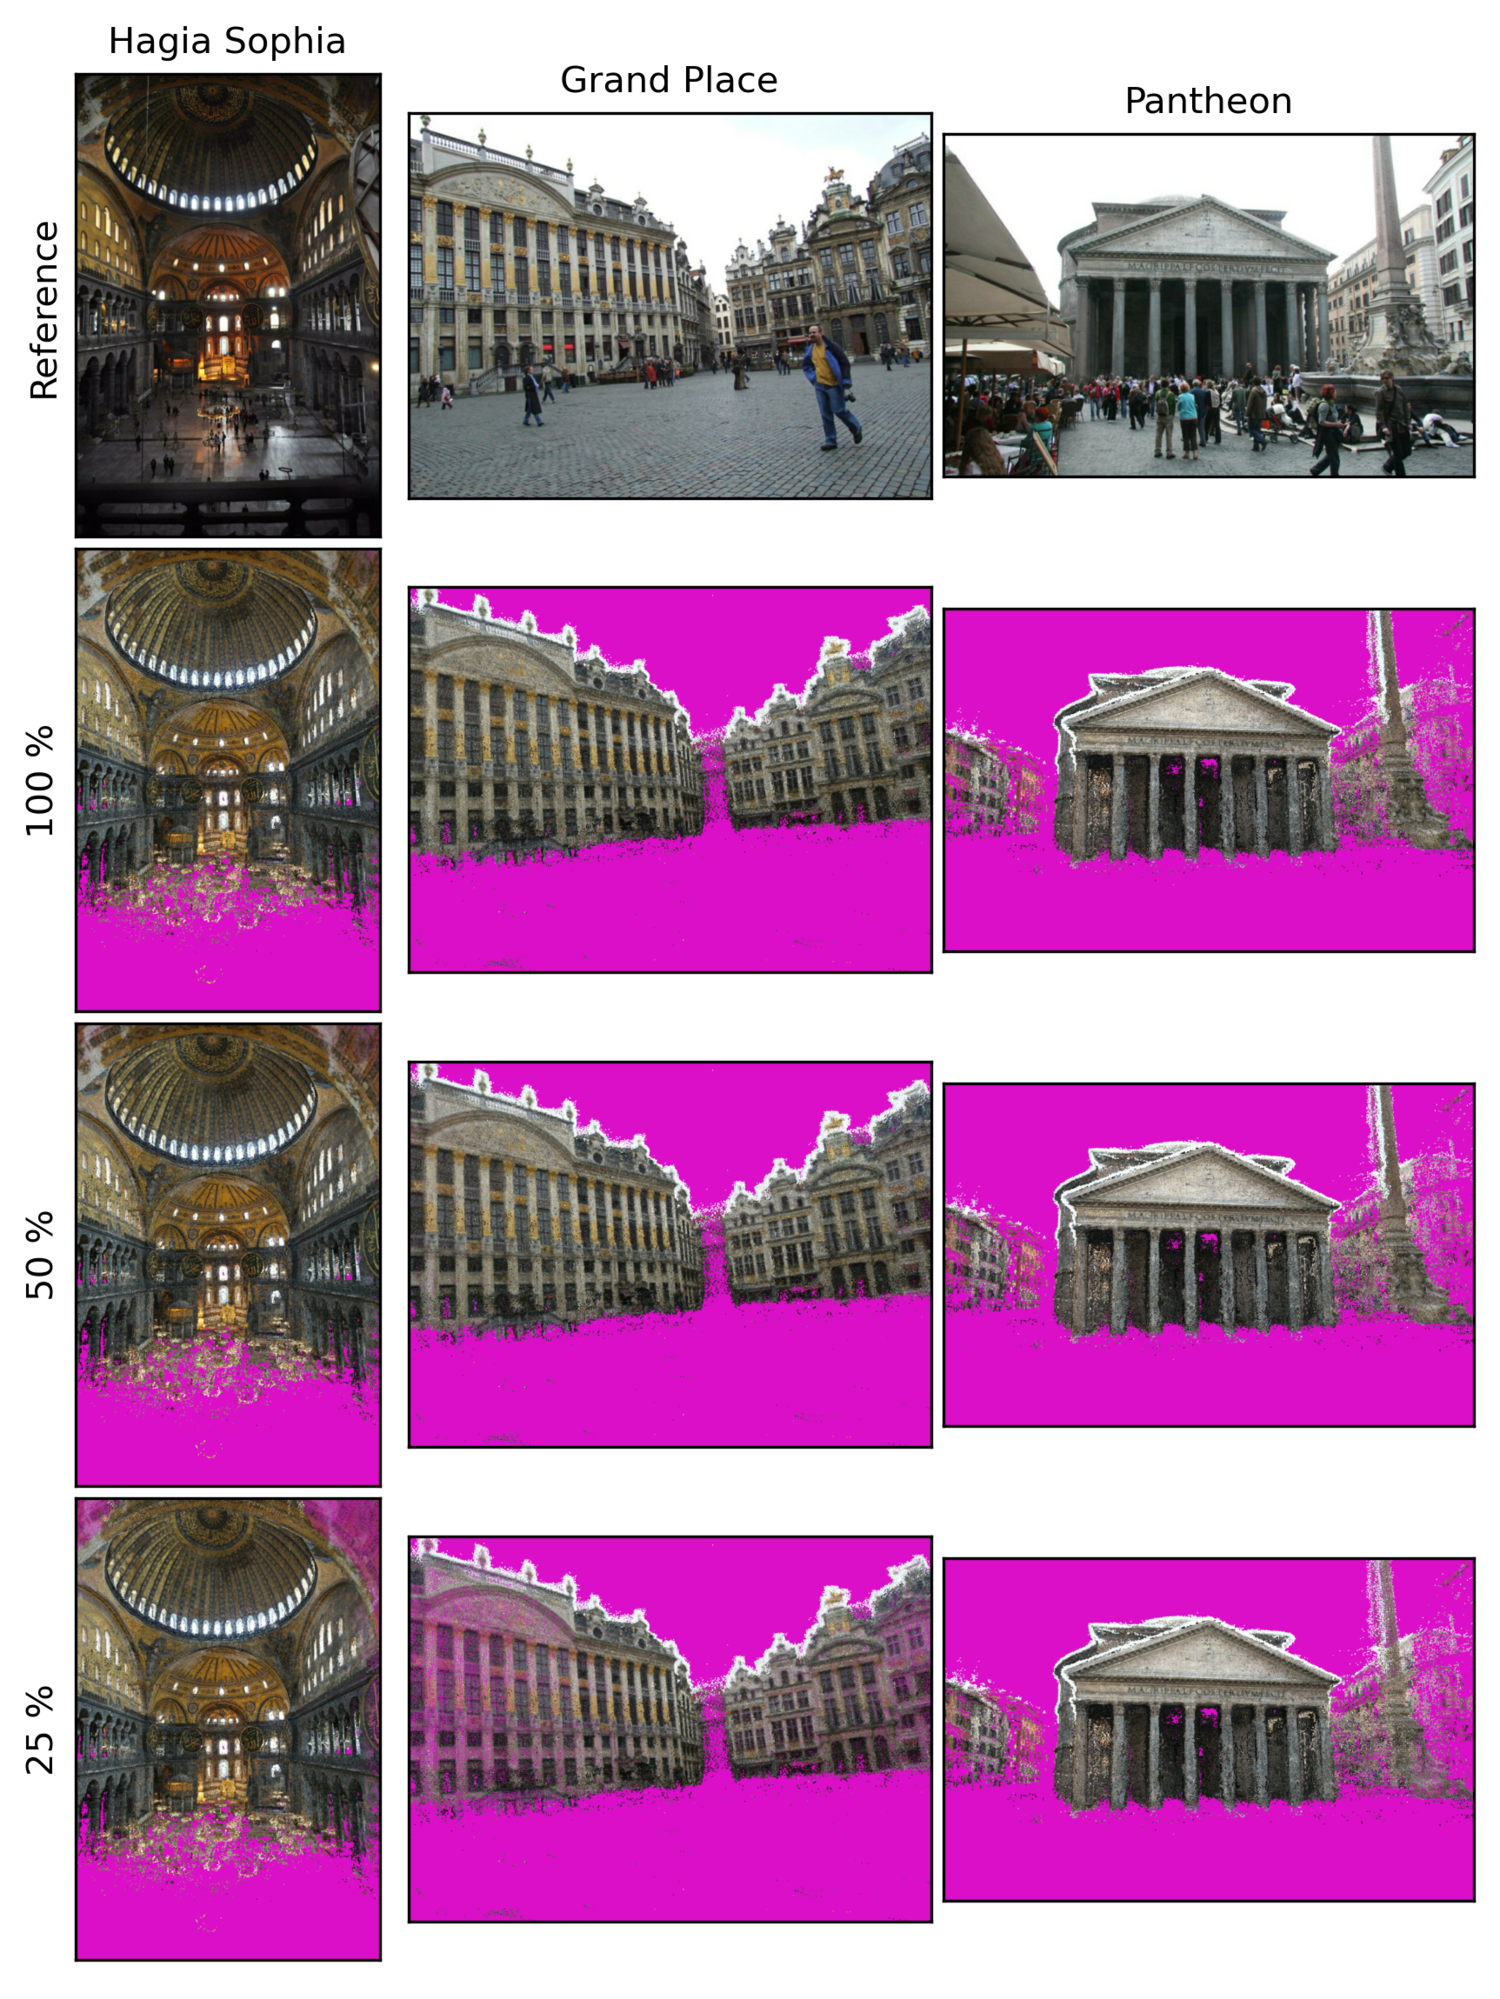
\includegraphics[width=0.95\textwidth]{graphics/pcd-all}
    \caption[Visual comparison of point cloud density influence on rendering]{
    Visual comparison of point cloud density influence on rendering.
    The renders are produced by Pyrender (\protect\UseVerb{term}) with contrastive
    background color to present the differences better. Point cloud
    simplification is done by Open3D's voxel downsampling to preserve the original
    structure with fewer points. The downsampling method proceeds in two steps;
    firstly, points are bucketed into 3D volumes called \emph{voxels},
    each resulting in exactly one point of the simplified output by averaging
    all points inside the source voxel in the second step. Since Pyrender
    has a fixed point size in screen space, its disadvantage can be seen---closest
    portions of the scene look sparser than the farther portions.}
    \label{fig:pcd_all}
\end{figure}

\begin{figure}
    \centering
    \includegraphics[width=0.9\textwidth]{graphics/hagia-renderers.png}
    \caption[Visual comparison of various renderers and point cloud
    densities for Hagia Sophia Collection]{Visual comparison of various
    renderers and point cloud densities for the Hagia Sophia Collection.
    Contrastive background color is displayed, Open3D's voxel downsampling is used
    for point cloud simplification.}
    \label{fig:hagia_renderers}
\end{figure}

\begin{figure}
    \centering
    \includegraphics[width=0.9\textwidth]{graphics/grand-renderers.png}
    \caption[Visual comparison of various renderers and point cloud
    densities for Grand Place Brussels Collection]{Visual comparison
    of various renderers and point cloud densities for Grand Place Brussels
    Collection. Contrastive background color is displayed, Open3D's
    voxel downsampling is used for point cloud simplification.}
    \label{fig:grand_renderers}
\end{figure}

\begin{figure}
    \centering
    \includegraphics[width=0.9\textwidth]{graphics/pantheon-renderers.png}
    \caption[Visual comparison of various renderers and point cloud
    densities for Pantheon Collection]{Visual comparison of various
    renderers and point cloud densities for Pantheon Collection.
    Contrastive background color is displayed, Open3D's voxel downsampling is used
    for point cloud simplification.}
    \label{fig:pantheon_renderers}
\end{figure}

Influence of the training data on outputs of the NRIW model is explored
in~\cref{fig:inloc_renderers})\footnotei{.}{As the ARTwin dataset is
not publicly available, it is excluded from visualizations here as its
display is minimized in the thesis.} Two views from the database are displayed
with all non-neural and neural renderers. In the first one with chairs,
one point with a comparatively larger diameter than most others is
near the left-down corner of the Splatter and Marcher image. These bigger splats
and spheres result in artifacts in neurally-generated images, as
depicted in the second image row. These patches are something that the screen space
renderer does not suffer from, as all points are of the same screen size.
The advantage of variable diameters
is visible in the second view. With the same  number of points,
the text on the board is sharper. Also, the floor gets some coverage
compared to the Pyrender-generated image. The background-filled portions of
Splatter-generated images are caused by the concrete actual point-splatting
implementation, both Splatter and Marcher use the same underlying diameters.\\

\begin{figure}
    \centering
    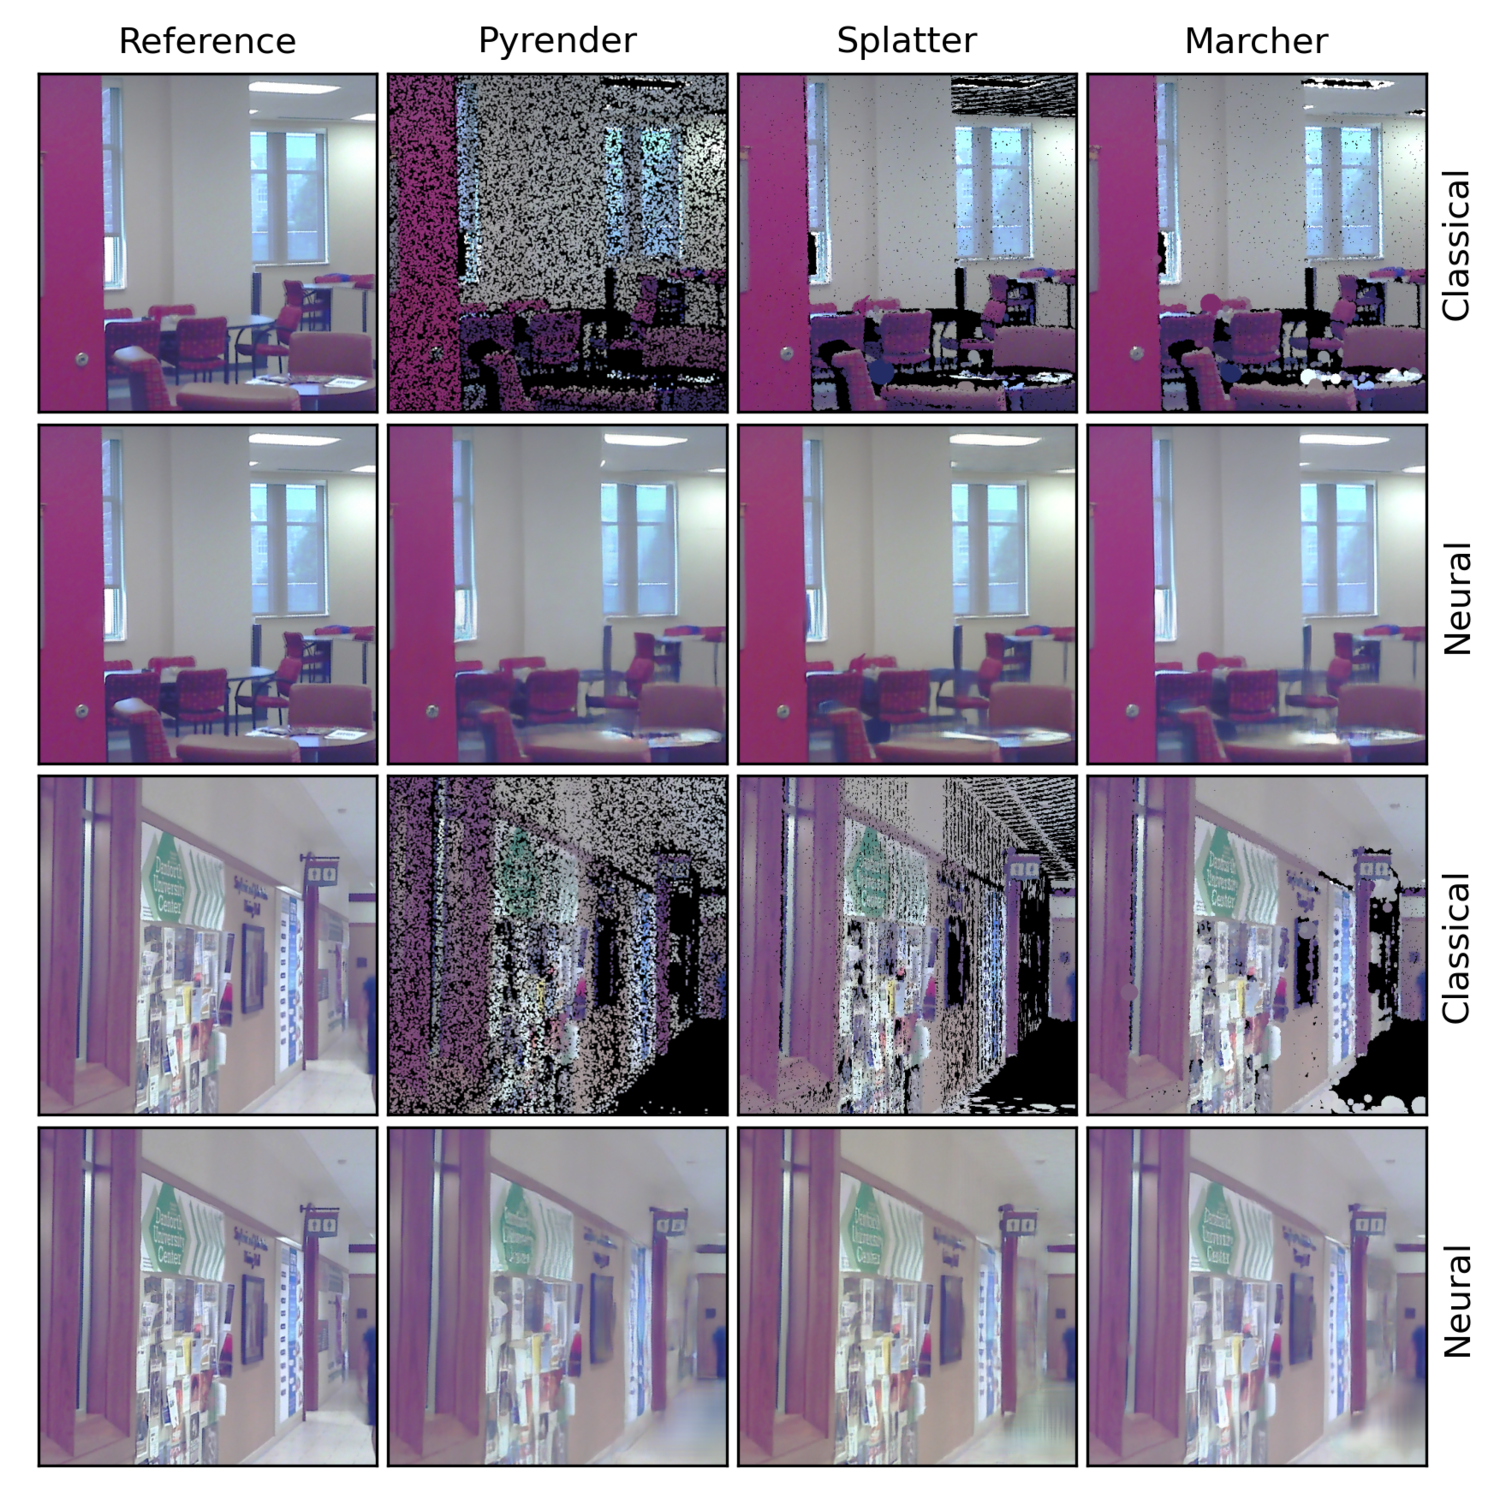
\includegraphics[width=0.9\textwidth]{graphics/inloc-renderers.png}
    \caption[Visual comparison of various renderers for InLoc dataset]{Visual
    comparison of various renderers for the InLoc dataset.
    For the indoor color profile, the default black background color is contrastive
    enough. The full point cloud was used for the visualizations. In the left-most
    column, repeated reference images for two different views are displayed. In the
    remaining columns, for a given view, up there always is an image generated by
    a non-neural type of renderer below which there is a render generated by NRIW
    trained on the data prepared by the respective non-neural renderer above.}
    \label{fig:inloc_renderers}
\end{figure}

The \textbf{computation rendering performance} relative comparison is
explored in~\cref{tab:render_times}. Relative because computational time
measurements are complex, and in a compute cluster environment that multiple
users actively use, they are also inherently affected by many
external entities. The influence can be alleviated to some extent by using proper
OS time measuring clock type, but it is always better to ideally use the
machine alone for the measuring task, which is hard to ensure on the cluster.
This complexity is to be seen in the table with times varying across
comparable output render dimensions and renderer types.

Across the datasets, the most consistent results are for \CC{} \emph{Splatter}
implementation. The smallest standard deviations show
implementation consistency. The point cloud size influence is also visible,
as for bigger renders and tens of millions of points, the rendering times
get considerably higher.

The second most consistent results are for
\emph{Pyrender} rendering that internally also uses the standard OpenGL
rendering pipeline and the standard and basic \verb|GL_POINTS| rendering
primitive. Since the implementation wrapper is in Python, we can see much
higher standard deviations.

From the \emph{neural} models, only one is picked for the measurements.
The model size and inference implementation are the same for a dataset, not
depending on the actual rendered data with which the model was trained. The times
are comparable, though the second biggest standard deviations can be seen.
The reason for shorter rendering times for the ARTwin dataset is unclear---the
implementation is in Python, using many software layers underneath, including
NVIDIA driver, so there may be the source of the difference,
alongside demonstrating the complexity of time measurements. The times
are considerably higher compared to those mentioned in the original paper,
but that is to be linked to much higher render dimensions. Moreover, the entire
neural rendering process includes rendering a given point cloud by some
non-neural renderer before inference occurs, which may even double the
rendering time in actual use cases.

\CC{} implementation of the Marcher does not use the standard OpenGL rendering
pipeline but CUDA parallelization over pixels. Most notably, it
iterates over points in the view frustum, so its rendering computational
performance depends on the 3D structure of a given view of the scene. The
view dependency is  visible in the table, as the standard deviations are
the biggest among renderer types. The implementation may hit some memory
caching or another problem around the InLoc database scan size, as the mean
rendering time and the standard deviation are orders
of magnitude higher than everything else.



\begin{table}
\caption[Mean rendering times]{Measured mean rendering times for the renderers,
collected with the thread CPU time clock, translating to the sum of
the system and user CPU time of the main thread from which rendering is
initiated. It does not include time elapsed during sleep, so it tries to avoid
measuring disturbance from other processes running on the CPU. The clock is
thus a rough approximation of what could be achieved when maximal
performance is sought, and a real-time OS is used. The neural model is not
distinguished here as the model size is the same even though tough weights vary
based on the training data used. The neural rendering time represents solely
the network inference, though preceding it, there must be an aligned triplet
generated, which includes invocation of some non-neural renderer that takes
also some time, as can be seen in the table. The dimension is the biggest
one present in the data being rendered. The measurements were taken on an
Intel Xeon E5-2698 and NVIDIA Tesla V100 GPU.}
\centering
    \begin{tabular}{l c c p{18mm} r r}
    \toprule
    Dataset & Points [M] & Dimension & Renderer & Time [ms] & $\sigma$ [ms] \\
    \midrule
    Hagia Sophia & 5  & 1248 & Neural   & 1\,361 & 139\\
                 &    &      & Pyrender &    783 & 111\\
                 &    &      & Splatter &    156 & 13  \\
                 &    &      & Marcher  & 1\,031 & 397\\[0.3cm]
    Grand Place  & 4  & 1168 & Neural   & 1\,280 & 147\\
                 &    &      & Pyrender &    679 & 82\\
                 &    &      & Splatter &    123 & 7\\
                 &    &      & Marcher  & 1\,448 & 570\\[0.3cm]
    Pantheon     & 5  & 1248 & Neural   & 1\,439 & 156\\
                 &    &      & Pyrender &    857 & 108\\
                 &    &      & Splatter &    173 & 4\\
                 &    &      & Marcher  &    446 & 127\\[0.3cm]
    ARTwin       & 27 & 1600 & Neural   &    871 & 140\\
                 &    &      & Pyrender & 1\,380 & 145\\
                 &    &      & Splatter & 1\,072 & 21\\
                 &    &      & Marcher  &    679 & 382\\[0.3cm]
    InLoc        & 40 & 1600 & Neural   & 1\,749 & 328\\
                 &    &      & Pyrender & 1\,447 & 93\\
                 &    &      & Splatter & 1\,340 & 51\\
                 &    &      & Marcher  & $2\,054\times10^3$ & $1\,684\times10^3$\\
    \bottomrule
    \end{tabular}
\label{tab:render_times}
\end{table}



\subsection{Comparison of localization approaches}

In the localization pipeline, XYZcuts are a vital part of the database
representation based on which a query image pose is calculated. Although
there are XYZcuts present in the InLoc raw dataset, for other datasets explored
in the thesis, they are not. Even for the InLoc dataset, some misalignments
are hidden in verified scan poses, also noted in the InLoc
algorithm Github repository issue. Thus, a way of computing this 3D data
representation is devised and applied to all datasets, including the InLoc one.
The process poses dependence of the localization
pipeline on a non-neural renderer---as specified in~\nameref{subsec:inloc},
the XYZcut is computed utilizing the depth map produced by a renderer per
localization database image. The depth map is used to transform
per-pixel 3D points placed on a default plane in the distance of one from a camera
center perpendicular to the given database image camera's optical axis.\\

In this section, three concepts are thus examined. Firstly, the influence
of a non-neural renderer-based database representation on the whole
localization process is explored on IMC image collections, end-to-end. Secondly,
the influence of given database representation with fixed pose verification step
renderer, including neural ones, on the localization performance is inspected
on ARTwin data. Finally, the influence of solely pose verification renderer
choice for one fixed database representation is considered for the InLoc dataset.\\

In~\cref{tab:imc_inloc_performance}, we can explore the localization on IMC
image collection from the smallest datasets on top to the biggest at the bottom of the
table. The overall rates of correctly localized queries are much smaller
compared to ARTwin and InLoc data. That may be caused by the combination of
three factors---several folds smaller dataset sizes; varying database image
dimensions, some of which are as small as 100~pixels in each dimension; varying
sensor types, sizes, and all adversarial effects of manual acquisition, such as
extensive blur. The absolute error sizes, when compared to the size of the
scene models, are relatively still small because, contrary to the other two
datasets, IMC data cover enormous external or internal spaces over much
bigger scale than mostly close looks at either manufacturing equipment or
corridors and other, in nature, office spaces.

The table shows that the splatting InLoc variant is predominantly the
most precise one with the most outliers on smaller precision thresholds
among the smallest Hagia Sophia collection. The second most precise
localization variant seems to be the Pyrender one. However, we will see that
comparison to the marching variant may be affected by a small dataset
size. The medians and means of Euclidean and angular distances support the
thesis of database size influence on localization performance (aside from the
simple idea that more database images mean a higher chance of retrieving one
captured more closely, thus triangulating a more precise pose). The bigger
the dataset size is, the smaller these statistics are. Also to be noted is the
fact that having fewer database images to perform the image retrieval has a
bigger influence on angular precision than Euclidean one.\\



\begin{table}
\caption[InLoc performance on IMC collections]{Evaluation
of localization performance on IMC collections using the InLoc
pipeline fully based on a given type of non-neural renderer,
including the pose verification step. The performance is
constituted by a percentual rate of correctly localized queries
at a given precision threshold. General statistics of calculated poses
in the form of mean and standard deviation for distance and
angular distance are also displayed.}
\centering
    \begin{tabular}{c c S[table-format=3.2] S[table-format=3.2] S[table-format=3.2] }
    \toprule
    Collection & Precision\,$+$\,Statistics & {Pyrender} & {Splatter} & {Marcher} \\
    \midrule
    Hagia Sophia
    & $\D2.50\m,\D7.5\dg$ &  \B{2}    &     0     &     0    \\
    & $\D5.00\m, 10.0\dg$ &  \B{4}    &  \B{4}    &     2    \\
    & $\D7.50\m, 15.0\dg$ &    18     &    16     & \B{20}   \\
    & $ 10.00\m, 20.0\dg$ & \B{52}    &    44     &    50    \\
    & $ 15.00\m, 30.0\dg$ &    86     & \B{90}    & \B{90}   \\
    & $ 20.00\m, 30.0\dg$ &    86     & \B{90}    & \B{90}   \\
    & Median [$\M$]       &     2.44  &  \B{2.10} &     2.37 \\
    & $\sigma$ [$\M$]     &     2.07  &  \B{1.80} &     2.21 \\
    & Median [$\dg$]      & \B{19.88} &    20.28  &    20.07 \\
    & $\sigma$ [$\dg$]    &    21.09  & \B{19.50} &    21.42 \\[0.3cm]
    Grand Place
    & $\D2.50\m,\D7.5\dg$ &     2    & \B{4}     &     2    \\
    & $\D5.00\m, 10.0\dg$ &     8    & \B{8}     &     6    \\
    & $\D7.50\m, 15.0\dg$ &    38    & \B{46}    & \B{46}   \\
    & $ 10.00\m, 20.0\dg$ &    72    & \B{76}    &    74    \\
    & $ 15.00\m, 30.0\dg$ & \B{90}   &    88     &    88    \\
    & $ 20.00\m, 30.0\dg$ & \B{90}   &    88     &    88    \\
    & Median [$\M$]       &     1.63 &  \B{1.50} &     1.75 \\
    & $\sigma$ [$\M$]     &     2.17 &  \B{1.45} &     2.29 \\
    & Median [$\dg$]      &    16.29 & \B{15.65} &    15.84 \\
    & $\sigma$ [$\dg$]    &    23.71 & \B{19.18} &    27.89 \\[0.3cm]
    Pantheon
    & $\D2.50\m,\D7.5\dg$ &     14     & \B{26}   &    22    \\
    & $\D5.00\m, 10.0\dg$ &     34     & \B{44}   & \B{44}   \\
    & $\D7.50\m, 15.0\dg$ &     72     & \B{82}   & \B{82}   \\
    & $ 10.00\m, 20.0\dg$ &     88     & \B{92}   &    90    \\
    & $ 15.00\m, 30.0\dg$ & \B{100}    &    98    &    96    \\
    & $ 20.00\m, 30.0\dg$ & \B{100}    &    98    &    96    \\
    & Median [$\M$]       &      1.50  & \B{1.09} &     1.48 \\
    & $\sigma$ [$\M$]     &      3.24  & \B{1.79} &     3.02 \\
    & Median [$\dg$]      &  \B{10.04} &   11.99  &    10.52 \\
    & $\sigma$ [$\dg$]    &     21.80  & \B{5.44} &    19.08 \\
    \bottomrule
    \end{tabular}
\label{tab:imc_inloc_performance}
\end{table}


Considering fixing the pose verification step and observing localization
performance with varying database representations,
\cref{tab:artwin_inloc_performance} presents the results on the ARTwin
dataset. The general positive impact of using neural rendering
approach for pose verification is shown. Across the pose verification
variants, the radii-based renderers perform better than the Pyrender ones,
no matter whether neural or non-neural variant is considered. This further
support the claim that better training data generation process positively affects
neural model performance, though the percentual margin may not be that
significant as these models can compensate for many imperfections in the
deep buffer.

Further, for the candidate pose generation InLoc localization
pipeline part, with a bigger dataset the marching-based InLoc Base variant
shows its better performance rather closing to the splatting variant, both
outperforming the Pyrender variant. From a median error point of view,
having a bigger dataset is also beneficial. The mean of median Euclidean
distance errors across the table is only $0.26\m$, and the mean of median
angular distance errors is as low as only $0.64\dg$. These results
are much better compared to those obtained on IMC collections, but as
described in the paragraphs devoted to~\cref{tab:imc_inloc_performance},
ARTwin dataset consists of more database images with the same dimensions,
consistent quality, and sensor parameters ensured by the image acquisition
process. The scanner used for dataset generation uses more \uv{normal} 2D
cameras to create $360\dg$ RGB scans, so when the InLoc database is created,
there are sometimes visible minor artifacts of this two-way process. An example
of such an artifact together with localization visualization is
in~\cref{fig:artwin_loc}. In the light of such minor defects, the absolute
errors are even more impressive.


\def\idone{$0.25\m, 2\dg$}
\def\idtwo{$0.50\m, 5\dg$}
\def\idthree{$5.00\m, 10\dg$}
\begin{table}
\caption[Pose verification performance on ARTwin dataset]{Evaluation
of localization performance on the ARTwin dataset. The performance is
constituted by a percentual rate of correctly localized queries
at a given precision threshold. InLoc Base refers to a renderer type on
which the localization database is constructed, pose verification renderer
is denoted as \emph{P} (Pyrender), \emph{S} (Splatter), \emph{M} (Marcher),
and three \emph{N} variants standing for NRIW trained on training data
generated by the respective renderer.}
\centering
    \begin{tabular}{l c S[table-format=3.2] S[table-format=3.2] S[table-format=3.2] }
    \toprule
    Pose Verification & InLoc Base & {\idone} & {\idtwo} & {\idthree} \\
    \midrule
    P   & Pyrender &    40.0  &    48.7  &    62.7  \\
        & Splatter & \B{40.1} & \B{49.9} &    62.6  \\
        & Marcher  &    39.9  &    49.2  & \B{63.1} \\[0.3cm]

    S   & Pyrender & \B{41.2} &    51.4  &    62.8  \\
        & Splatter &    40.0  &    53.3  & \B{64.7} \\
        & Marcher  &    40.9  & \B{53.5} &    63.9  \\[0.3cm]

    M   & Pyrender &    41.0  &    50.7  &    65.3  \\
        & Splatter & \B{42.1} & \B{53.1} & \B{65.8} \\
        & Marcher  &    41.3  &    52.7  &    65.5  \\[0.3cm]

    N-P & Pyrender &    43.8  &    51.9  &    68.3  \\
        & Splatter &    44.0  &    51.8  & \B{70.1} \\
        & Marcher  & \B{44.2} & \B{52.8} &    69.2  \\[0.3cm]

    N-S & Pyrender &    45.6  &    55.1  &    72.7  \\
        & Splatter & \B{45.9} &    59.3  &    73.4  \\
        & Marcher  &    45.7  & \B{59.5} & \B{74.6} \\[0.3cm]

    N-M & Pyrender &    45.9  &    55.0  &    71.9  \\
        & Splatter &    46.2  & \B{60.5} &    73.8  \\
        & Marcher  & \B{47.2} &    58.9  & \B{74.7} \\
    \bottomrule
    \end{tabular}
\label{tab:artwin_inloc_performance}
\end{table}

\begin{figure}
    \centering
    \begin{subfigure}{.95\textwidth}
          \centering
       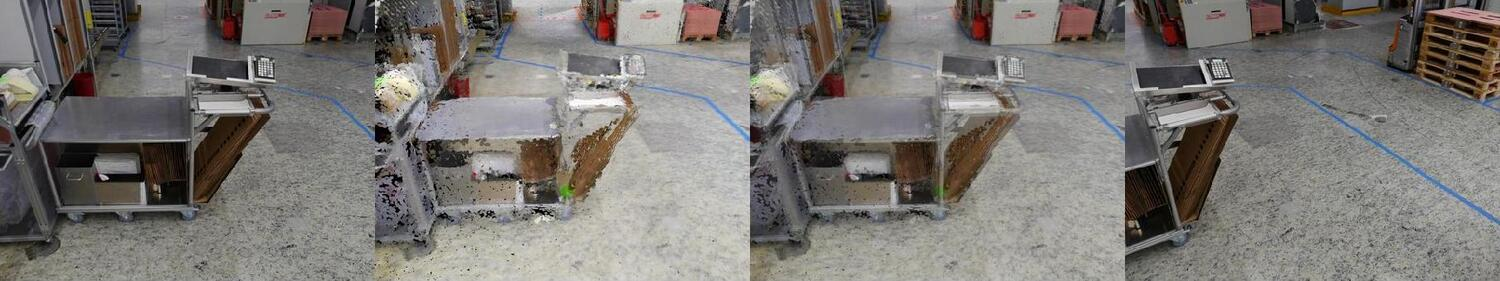
\includegraphics[width=.95\textwidth]{../graphics/err_0.01m_0deg_results_q_id_3_best_db_1}
    \end{subfigure}%

    \begin{subfigure}[width=.95\textwidth]{.95\textwidth}
          \centering
          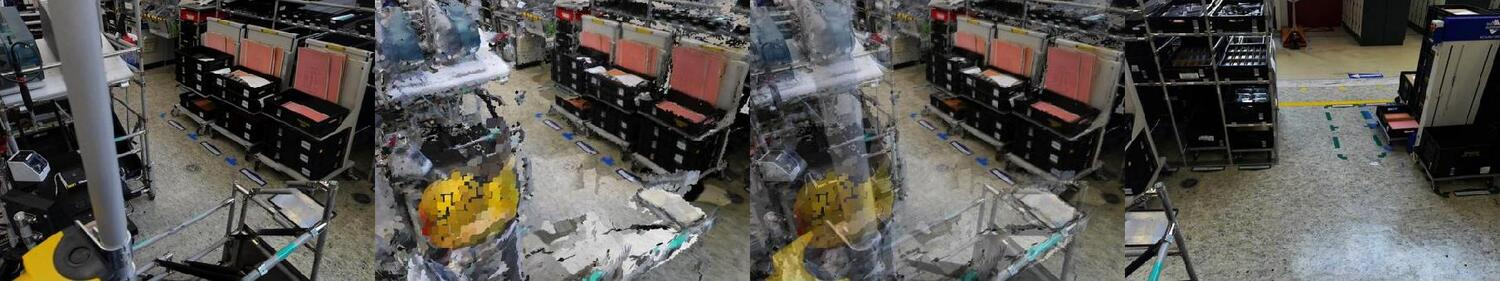
\includegraphics[width=.95\textwidth]{../graphics/err_0.18m_1deg_results_q_id_137_best_db_1}
    \end{subfigure}
    \caption[Sample localization visualizations]{The first column shows the
    query photo, the second render of the best candidate position, the third
    a blend of the two preceding columns and the last column shows the
    database photo obtained from the image retrieval step. The upper row
    shows an error of $0.01\m$ and $0\dg$, the second an error of $0.18\m$
    and~$1\dg$. On the query image of the second row, there is also visible
    the relic of the reprojection from panorama photo to 2D photo on the tubes
    in the foreground.
    }\label{fig:artwin_loc}
\end{figure}



% \begin{figure}
%     \centering
%     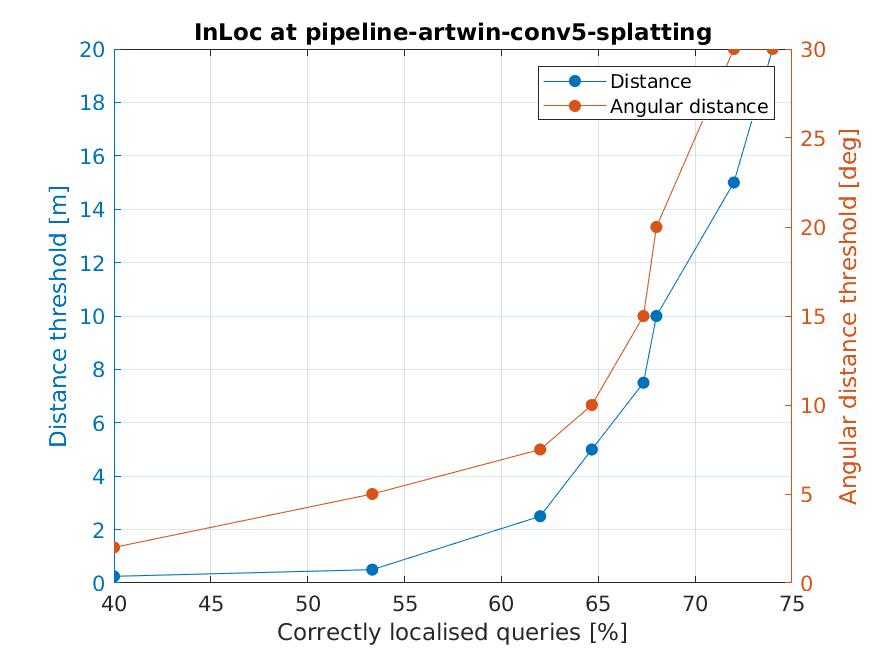
\includegraphics[width=.95\textwidth]{graphics/correctly_localized_queries}
%     \caption[]{}
%     \label{fig:artwin_loc_graph}
% \end{figure}


Finally, for the InLoc dataset, the results are presented
in~\cref{tab:inloc_performance}. The percentual rates are comparatively
worse than the one from previous research; the reason is that I faced
a lot of issues around the InLoc dataset, including the mentioned skewed
database positions, and I was not able to resolve it properly.
Though lower in absolute numbers, the distortion is the same across
all results; thus, the relative comparisons still pose valuable insights.
Based on the outcomes of preceding experiments, with fixed localization
dataset generation via splatting, we compare the performance of various
pose verification approaches on the page \url{https://www.visuallocalization.net}.

For the InLoc dataset, the Marcher renderer performs best, outperforming
both remaining non-neural renderers. The dominance over this dataset
gets translated over to neural models as well. Even more than in the case
of the ARTwin dataset, we can see the benefit of neural rendering in this
case: ray marching varies between 7.1~\% to 9.1~\% for three precision
thresholds. All three neural models show a positive impact over non-neural
variants.

The splatting-based variants are the least performing among others on this
dataset. The reason may be hidden in Lipponer's implementation, as
some artifacts are visible in~\cref{fig:inloc_renderers}. That may
arise from the number of points in the scan, as it is the highest among all
the datasets in the thesis, or the format of the scans themselves, generated
by Matlab in the raw dataset data and later transformed into PLY file format.

Despite all the complications with the InLoc dataset, radii-based renderers
shown their value and benefits over all datasets, as well as neural rendering
that further pushes localization performance rates.



\begin{table}
\caption[InLoc performance on InLoc dataset]{Percentual rate of
correctly localized query images within the displayed distance
and angular distance for the DUC1 floor. The table explores the behavior
of fixed candidate positions localization part and multiple
pose verification rendering methods denoted as \emph{P} (Pyrender),
\emph{S} (Splatter), \emph{M} (Marcher), and three \emph{N} variants
standing for NRIW trained on training data generated by the respective
renderer.}
\centering
    \begin{tabular}{c S[table-format=3.2] S[table-format=3.2] S[table-format=3.2] | S[table-format=3.2] S[table-format=3.2] S[table-format=3.2] }
    \toprule
    Rate [\%]           & {P}  & {S}  & {M}     & {N-P} & {N-S} & {N-M} \\
    \midrule
    $\D0.25\m,\D2.0\dg$ & 22.2 & 19.2 & \B{22.7} & 26.8 & 21.2 & \B{29.8} \\
    $\D0.50\m,\D5.0\dg$ & 28.3 & 26.3 & \B{30.3} & 31.8 & 24.2 & \B{38.9} \\
    $\D5.00\m, 10.0\dg$ & 37.4 & 36.4 & \B{41.9} & 43.4 & 31.8 & \B{51.0} \\
    \bottomrule
    \end{tabular}
\label{tab:inloc_performance}
\end{table}

\chapter*{Conclusion}
\addcontentsline{toc}{chapter}{Conclusion}

This thesis examines the usage of various rendering techniques in the InLoc
algorithm solving the visual localization problem and its verification step.
The point cloud rendering approaches, and later localization performance are
evaluated on three different dataset types covering both exteriors and
interiors; the InLoc implementation is generalized so that a general dataset,
not only the one that InLoc was released with, can be inputted for localization.

Four different rendering approaches are utilized---as a baseline approach,
the default OpenGL point rendering primitive \verb|GL_POINTS| is used, further,
point splatting and ray marching with signed distance fields are explored.
Finally, aside from the three classical rendering approaches, a neural
rendering deep neural network model is compared with the previous ones. As not
all mentioned renderers were in existence prior to the thesis with sufficient
performance to be able to render point clouds of sizes present in the datasets,
third-party point splatting C++ implementation within a graphical interface is
enhanced with headless rendering capabilities, the capability to read external point
clouds and camera parameters, and output depth information for renders. The ray
marching renderer is implemented in C++ and CUDA from the ground, eventually
reusing the same components from the splatter enhancements. To the best of our knowledge,
previously, there were no such implementations with these capabilities being able
to render tens of millions of points in a reasonable time.\\

We considered the renderers from various angles---rendering performance from visual
and statistical perspective, from computational performance, and finally, from
influence on the localization performance. We show that aside from computational
perspective, the four renderers split roughly into three groups: the predominantly
least performant algorithm is Pyrender, followed by the Splatter and Marcher
implementations with the NRIW model on the top.

\emph{Pyrender} suffers from its slower
implementation in Python and from the primitive it uses as the points have fixed
size in the screen space, which defies perspective drawing principles, leading to
visual artifacts in the form of occlusion problems.

\emph{Splatter} and \emph{Marcher} are less easy to separate. Their principle
is similar as it uses diameters assigned to points and renders them as splats or
spheres. In practical use cases, there are differences, however.
The Splatter requires a normal vector per point on top of diameters to
properly put a face to the splats. In the case of all datasets explored in the
thesis, we did not encounter a situation where a dataset would simultaneously
explore one space from the inside and outside. However, if this happens, Splatter
would require additional functionality to dynamically compute normals per view
or switch directions based on some condition fulfillment. On the other hand,
Splatter shows less dependency on the view frustum contents, whereas Marcher
performs much less consistently. For some views, the rendering time may be
considerably longer than for others. There is room for improvements in the
implementation that may mitigate this issue, including the possible memory caching
boundary hit, causing extremely prolonged rendering times in some cases. Visually,
Splatter can represent corners and edges with less blur. Finally, both
renderers increase the performance of the InLoc pipeline when used for the
dataset's transformation into the InLoc format and for training a neural model
used in the verification step.

The \emph{NRIW} model further pushes localization performance due to its more
realistically-looking rendering capabilities that get exploited in the verification
step of the localization pipeline. The disadvantages and the price for the localization
precision gains are speed, as the model needs, on top of its own slower runtime,
a proxy render of a point cloud from a candidate position generated by another
non-neural renderer, and also its scene dependency that requires training for
every dataset explored. There has been considerable progress in the neural rendering
field since work on the thesis started, so future work may explore these advancements.\\

To summarize, when maximal localization performance is sought, Splatter and Marcher
help the localization pipeline's frontend, together with neural rendering based on the
same. For concrete use cases, other differentiating factors can help to choose a specific
renderer. When the time of answering a localization query is to be minimized, it may be
worth sacrificing some precision by either using the non-neural renderers for the whole
pipeline or, as we show, by lowering the number of points in the scene model that is from
both statistical and visual point of view comparable with the advantage of faster
rendering times. Future work may analyze the effect of lowering the resolution of the
database and query images to inspect the computational performance further.



%%% Bibliography
%%% Bibliography (literature used as a source)
%%%
%%% We employ bibTeX to construct the bibliography. It processes
%%% citations in the text (e.g., the \cite{...} macro) and looks up
%%% relevant entries in the bibliography.bib file.
%%%
%%% The \bibliographystyle command selects, which style will be used
%%% for references from the text. The argument in curly brackets is
%%% the name of the corresponding style file (*.bst). Both styles
%%% mentioned in this template are included in LaTeX distributions.

% \bibliographystyle{apalike}
% \bibliographystyle{dinat}
\bibliographystyle{plainnat}    %% Author (year)
% \bibliographystyle{unsrt}     %% [number]

\renewcommand{\bibname}{Bibliography}

%%% Generate the bibliography. Beware that if you cited no works,
%%% the empty list will be omitted completely.

\bibliography{bibliography}

%%% If case you prefer to write the bibliography manually (without bibTeX),
%%% you can use the following. Please follow the ISO 690 standard and
%%% citation conventions of your field of research.

% \begin{thebibliography}{99}
%
% \bibitem{lamport94}
%   {\sc Lamport,} Leslie.
%   \emph{\LaTeX: A Document Preparation System}.
%   2nd edition.
%   Massachusetts: Addison Wesley, 1994.
%   ISBN 0-201-52983-1.
%
% \end{thebibliography}


%%% Figures used in the thesis (consider if this is needed)
\listoffigures

%%% Tables used in the thesis (consider if this is needed)
%%% In mathematical theses, it could be better to move the list of tables to the beginning of the thesis.
\listoftables

%%% Abbreviations used in the thesis, if any, including their explanation
%%% In mathematical theses, it could be better to move the list of abbreviations to the beginning of the thesis.
\chapwithtoc{List of Abbreviations}
\begin{acronym}
 \acro{CG}{Computer Graphics}
 \acro{CNN}{Convolutional Neural Network}
 \acro{CSG}{Constructive Solid Geometry}
 \acro{CV}{Computer Vision}
 \acro{DB}{Database}
 \acro{DNN}{Deep Neural Network}
 \acro{EWA}{Elliptical Weighted Average}
 \acro{FoV}{Field of View}
 \acro{GAN}{Generative Adversarial Networks}
 \acro{GPU}{Graphics Processing Unit}
 \acro{IMC}{Image Matching Challenge}
 \acro{MVS}{MultiView Stereo}
 \acro{NN}{Neural Network}
 \acro{NRIW}{Neural Rerendering in the Wild}
 \acro{OS}{Operating System}
 \acro{RGB(D)}{Red Green Blue (Depth)}
 \acro{SDF}{Signed Distance Functions}
 \acro{SfM}{Structure from Motion}
 \acro{VAE}{Variational Autoencoder}
 \acro{VGG}{Visual Geometry Group}
\end{acronym}

%%% Attachments to the master thesis, if any. Each attachment must be
%%% referred to at least once from the text of the thesis. Attachments
%%% are numbered.
%%%
%%% The printed version should preferably contain attachments, which can be
%%% read (additional tables and charts, supplementary text, examples of
%%% program output, etc.). The electronic version is more suited for attachments
%%% which will likely be used in an electronic form rather than read (program
%%% source code, data files, interactive charts, etc.). Electronic attachments
%%% should be uploaded to SIS and optionally also included in the thesis on a~CD/DVD.
%%% Allowed file formats are specified in provision of the rector no. 72/2017.
%\appendix
%\chapter{Attachments}

%\section{First Attachment}

\openright
\end{document}
